% Options for packages loaded elsewhere
\PassOptionsToPackage{unicode}{hyperref}
\PassOptionsToPackage{hyphens}{url}
%
\documentclass[
]{article}
\usepackage{amsmath,amssymb}
\usepackage{iftex}
\ifPDFTeX
  \usepackage[T1]{fontenc}
  \usepackage[utf8]{inputenc}
  \usepackage{textcomp} % provide euro and other symbols
\else % if luatex or xetex
  \usepackage{unicode-math} % this also loads fontspec
  \defaultfontfeatures{Scale=MatchLowercase}
  \defaultfontfeatures[\rmfamily]{Ligatures=TeX,Scale=1}
\fi
\usepackage{lmodern}
\ifPDFTeX\else
  % xetex/luatex font selection
\fi
% Use upquote if available, for straight quotes in verbatim environments
\IfFileExists{upquote.sty}{\usepackage{upquote}}{}
\IfFileExists{microtype.sty}{% use microtype if available
  \usepackage[]{microtype}
  \UseMicrotypeSet[protrusion]{basicmath} % disable protrusion for tt fonts
}{}
\makeatletter
\@ifundefined{KOMAClassName}{% if non-KOMA class
  \IfFileExists{parskip.sty}{%
    \usepackage{parskip}
  }{% else
    \setlength{\parindent}{0pt}
    \setlength{\parskip}{6pt plus 2pt minus 1pt}}
}{% if KOMA class
  \KOMAoptions{parskip=half}}
\makeatother
\usepackage{xcolor}
\usepackage[margin=1in]{geometry}
\usepackage{graphicx}
\makeatletter
\def\maxwidth{\ifdim\Gin@nat@width>\linewidth\linewidth\else\Gin@nat@width\fi}
\def\maxheight{\ifdim\Gin@nat@height>\textheight\textheight\else\Gin@nat@height\fi}
\makeatother
% Scale images if necessary, so that they will not overflow the page
% margins by default, and it is still possible to overwrite the defaults
% using explicit options in \includegraphics[width, height, ...]{}
\setkeys{Gin}{width=\maxwidth,height=\maxheight,keepaspectratio}
% Set default figure placement to htbp
\makeatletter
\def\fps@figure{htbp}
\makeatother
\setlength{\emergencystretch}{3em} % prevent overfull lines
\providecommand{\tightlist}{%
  \setlength{\itemsep}{0pt}\setlength{\parskip}{0pt}}
\setcounter{secnumdepth}{-\maxdimen} % remove section numbering
\newlength{\cslhangindent}
\setlength{\cslhangindent}{1.5em}
\newlength{\csllabelwidth}
\setlength{\csllabelwidth}{3em}
\newlength{\cslentryspacingunit} % times entry-spacing
\setlength{\cslentryspacingunit}{\parskip}
\newenvironment{CSLReferences}[2] % #1 hanging-ident, #2 entry spacing
 {% don't indent paragraphs
  \setlength{\parindent}{0pt}
  % turn on hanging indent if param 1 is 1
  \ifodd #1
  \let\oldpar\par
  \def\par{\hangindent=\cslhangindent\oldpar}
  \fi
  % set entry spacing
  \setlength{\parskip}{#2\cslentryspacingunit}
 }%
 {}
\usepackage{calc}
\newcommand{\CSLBlock}[1]{#1\hfill\break}
\newcommand{\CSLLeftMargin}[1]{\parbox[t]{\csllabelwidth}{#1}}
\newcommand{\CSLRightInline}[1]{\parbox[t]{\linewidth - \csllabelwidth}{#1}\break}
\newcommand{\CSLIndent}[1]{\hspace{\cslhangindent}#1}
\usepackage{pdflscape}
\newcommand{\blandscape}{\begin{landscape}}
\newcommand{\elandscape}{\end{landscape}}
\usepackage{booktabs}
\usepackage{caption}
\usepackage{longtable}
\ifLuaTeX
  \usepackage{selnolig}  % disable illegal ligatures
\fi
\IfFileExists{bookmark.sty}{\usepackage{bookmark}}{\usepackage{hyperref}}
\IfFileExists{xurl.sty}{\usepackage{xurl}}{} % add URL line breaks if available
\urlstyle{same}
\hypersetup{
  pdftitle={Supplementary Material},
  hidelinks,
  pdfcreator={LaTeX via pandoc}}

\title{Supplementary Material}
\usepackage{etoolbox}
\makeatletter
\providecommand{\subtitle}[1]{% add subtitle to \maketitle
  \apptocmd{\@title}{\par {\large #1 \par}}{}{}
}
\makeatother
\subtitle{Seabird assemblages are linked to the major western boundary
current off eastern Australia}
\author{}
\date{\vspace{-2.5em}2023-10-18}

\begin{document}
\maketitle

This document is an accompanying file for \textbf{XXXXX et al.~(2023)
Divers. Distr.}. Briefly, here you will find --

\begin{itemize}
\tightlist
\item
  \textbf{List of packages} and version used for data wrangling,
  visualisation and analyses;
\item
  \textbf{Table S1}: Summary of sampling effort by voyage;
\item
  \textbf{Figure S1}: Number of occurrence, frequency of occurrence
  (FO), and numeric frequency (NF) by season;
\item
  \textbf{Figure S2}: Species richness and total number of seabirds
  counted by grid/season;
\item
  \textbf{Figure S3}: Plots for choosing best RCP group number
  (\texttt{multifit});
\item
  \textbf{Figure S4}: Residual plots from the best fitted models;
\item
  \textbf{Figure S5}: Partial plots for covariates;
\item
  \textbf{Figure S6}: Probability maps from seasonal predictions;
\item
  \textbf{Figure S7}: Species profiles for each season;
\item
  \textbf{Figure S8}: Species-richness and sample-coverage curves.
\end{itemize}

\newpage

\hypertarget{list-of-packages}{%
\section{List of packages}\label{list-of-packages}}

We used the following packages `plyr' 1.8.8 (Wickham, 2011), `dplyr'
1.1.2 (Wickham, François, et al., 2023), `tidyr' 1.3.0 (Wickham,
Vaughan, et al., 2023), `readr' 2.1.4 (Wickham, Hester, et al., 2023),
`tibble' 3.2.1 (Müller \& Wickham, 2023), `lubridate' 1.9.2 (Grolemund
\& Wickham, 2011), `stringr' 1.5.0 (Wickham, 2022), `purrr' 1.0.1
(Wickham \& Henry, 2023), `ggplot2' 3.4.2 (Wickham, 2016), `ggspatial'
1.1.7 (Dunnington, 2022), `patchwork' 1.1.2 (Pedersen, 2022),
`RColorBrewer' 1.1-3 (Neuwirth, 2022), `rnaturalearth' 0.3.2 (Massicotte
\& South, 2023), `sp' 1.6-0 (Bivand et al., 2013; E. J. Pebesma \&
Bivand, 2005), `sf' 1.0-8 (E. Pebesma, 2018), `mapview' 2.11.0
(Appelhans et al., 2022), `raster' 3.5-21 (Hijmans, 2022a), `terra'
1.6-7 (Hijmans, 2022b), `rerddap' 1.0.2 (Chamberlain, 2023),
`rerddapXtracto' 1.1.4 (Mendelssohn, 2022), `hadsstR' (Byrnes \& Dunic,
2017), `corrplot' 0.92 (Wei \& Simko, 2021), and the ones referenced in
the main text.

The code is archived in a repository \textbf{(Zenodo repo)}, and you can
find a detailed walk-through in it.

\newpage

\begin{landscape}

\begin{longtable}{lrrllrrr}
\caption*{
{\large \textbf{TABLE S1.} Summary of seabird sampling effort by voyage, off eastern Australia, during Australasian Seabird Group's ship-based surveys between 2016--2021. Start and finish dates and geographic ranges of each voyage, including the number of seabird records and the number of individuals and species recorded}
} \\ 
\toprule
\textbf{Voyage} & \textbf{Date start} & \textbf{Date end} & \textbf{Latitudinal range} & \textbf{Longitudinal range} & \textbf{No. of records} & \textbf{No. of birds} & \textbf{No. of species} \\ 
\midrule
in2016\_t02 & 2016-08-25 & 2016-08-28 & -43 – -34 & 147 – 152 & 344 & 475 & 25 \\ 
in2016\_v06 & 2016-10-29 & 2016-11-12 & -27 – -27 & 153 – 155 & 284 & 2892 & 14 \\ 
in2017\_v02 & 2017-03-16 & 2017-03-27 & -47 – -43 & 142 – 147 & 911 & 7122 & 30 \\ 
in2017\_t01 & 2017-09-24 & 2017-10-01 & -33 – -9 & 143 – 154 & 370 & 4540 & 17 \\ 
in2017\_t02 & 2017-11-24 & 2017-11-25 & -44 – -42 & 141 – 147 & 113 & 11010 & 17 \\ 
in2018\_t02 & 2018-05-14 & 2018-05-20 & -43 – -27 & 148 – 154 & 214 & 6168 & 31 \\ 
in2018\_c01 & 2018-05-28 & 2018-06-07 & -41 – -39 & 146 – 149 & 644 & 2846 & 25 \\ 
in2018\_v04 & 2018-09-11 & 2018-10-07 & -47 – -34 & 141 – 155 & 1136 & 10434 & 36 \\ 
in2018\_v06 & 2018-11-22 & 2018-12-18 & -44 – -41 & 146 – 149 & 1957 & 59628 & 43 \\ 
in2019\_v07 & 2019-04-10 & 2019-04-22 & -43 – -38 & 147 – 150 & 412 & 1472 & 26 \\ 
in2019\_t01 & 2019-04-29 & 2019-05-02 & -44 – -39 & 141 – 148 & 140 & 177 & 18 \\ 
in2019\_v04 & 2019-08-07 & 2019-09-01 & -24 – -10 & 146 – 160 & 1321 & 13383 & 26 \\ 
in2019\_t02 & 2019-10-03 & 2019-10-10 & -27 – -9 & 142 – 154 & 245 & 1895 & 28 \\ 
fk201228 & 2020-12-27 & 2021-01-25 & -27 – -23 & 153 – 157 & 1063 & 17298 & 20 \\ 
fk210206 & 2021-02-06 & 2021-03-05 & -27 – -19 & 153 – 157 & 1107 & 3306 & 14 \\ 
\bottomrule
\end{longtable}

\newpage

\begin{figure}
\centering
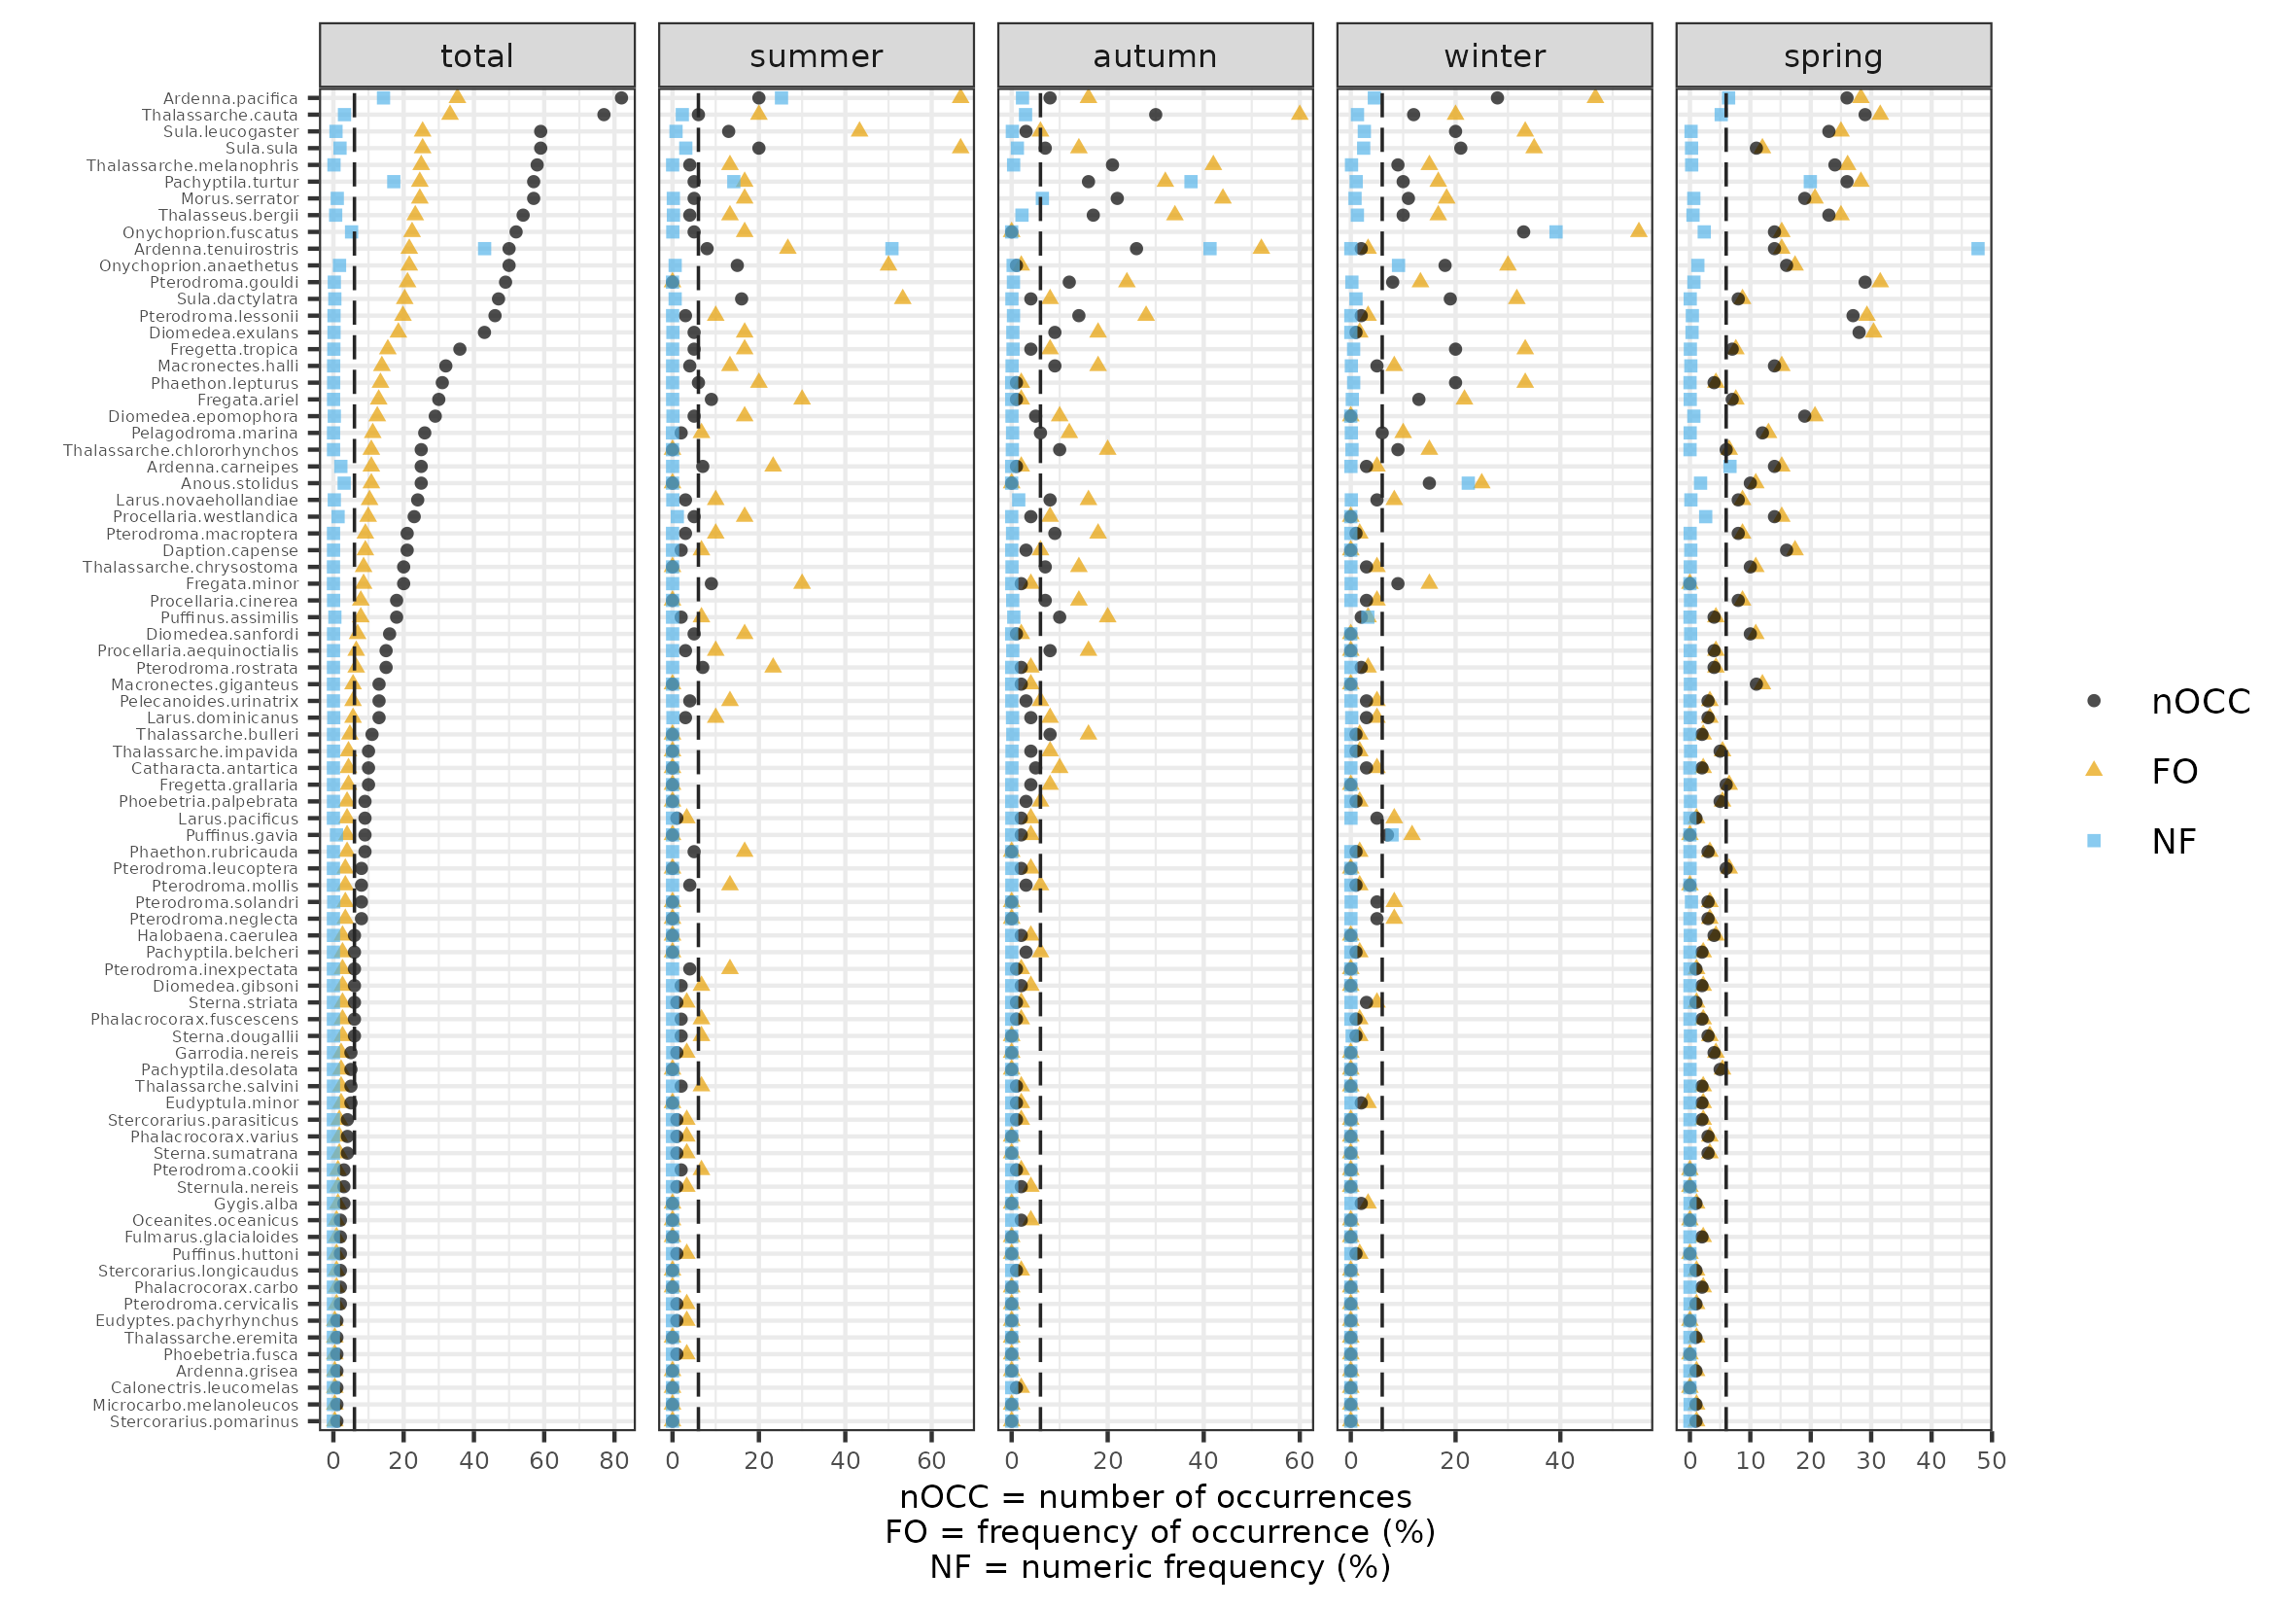
\includegraphics{../results/FigS1_spp-nOCC-FO-NF-seasons.png}
\caption{\textbf{Figure S1.} Number of occurrences (nOCC), frequency of
occurrence (FO) and numeric frequency (NF) of seabirds recorded off
eastern Australia during Australasian Seabird Group's ship-based surveys
between 2016--2021. The dashed line represents the number of occurrence
thresholds (n = 6) each taxon had to match for its inclusion in the
seasonal models (see \emph{Methods} in the main text). Species are
ordered from the largest to the lowest total number of occurrences.}
\end{figure}

\end{landscape}

\newpage

\begin{figure}
\centering
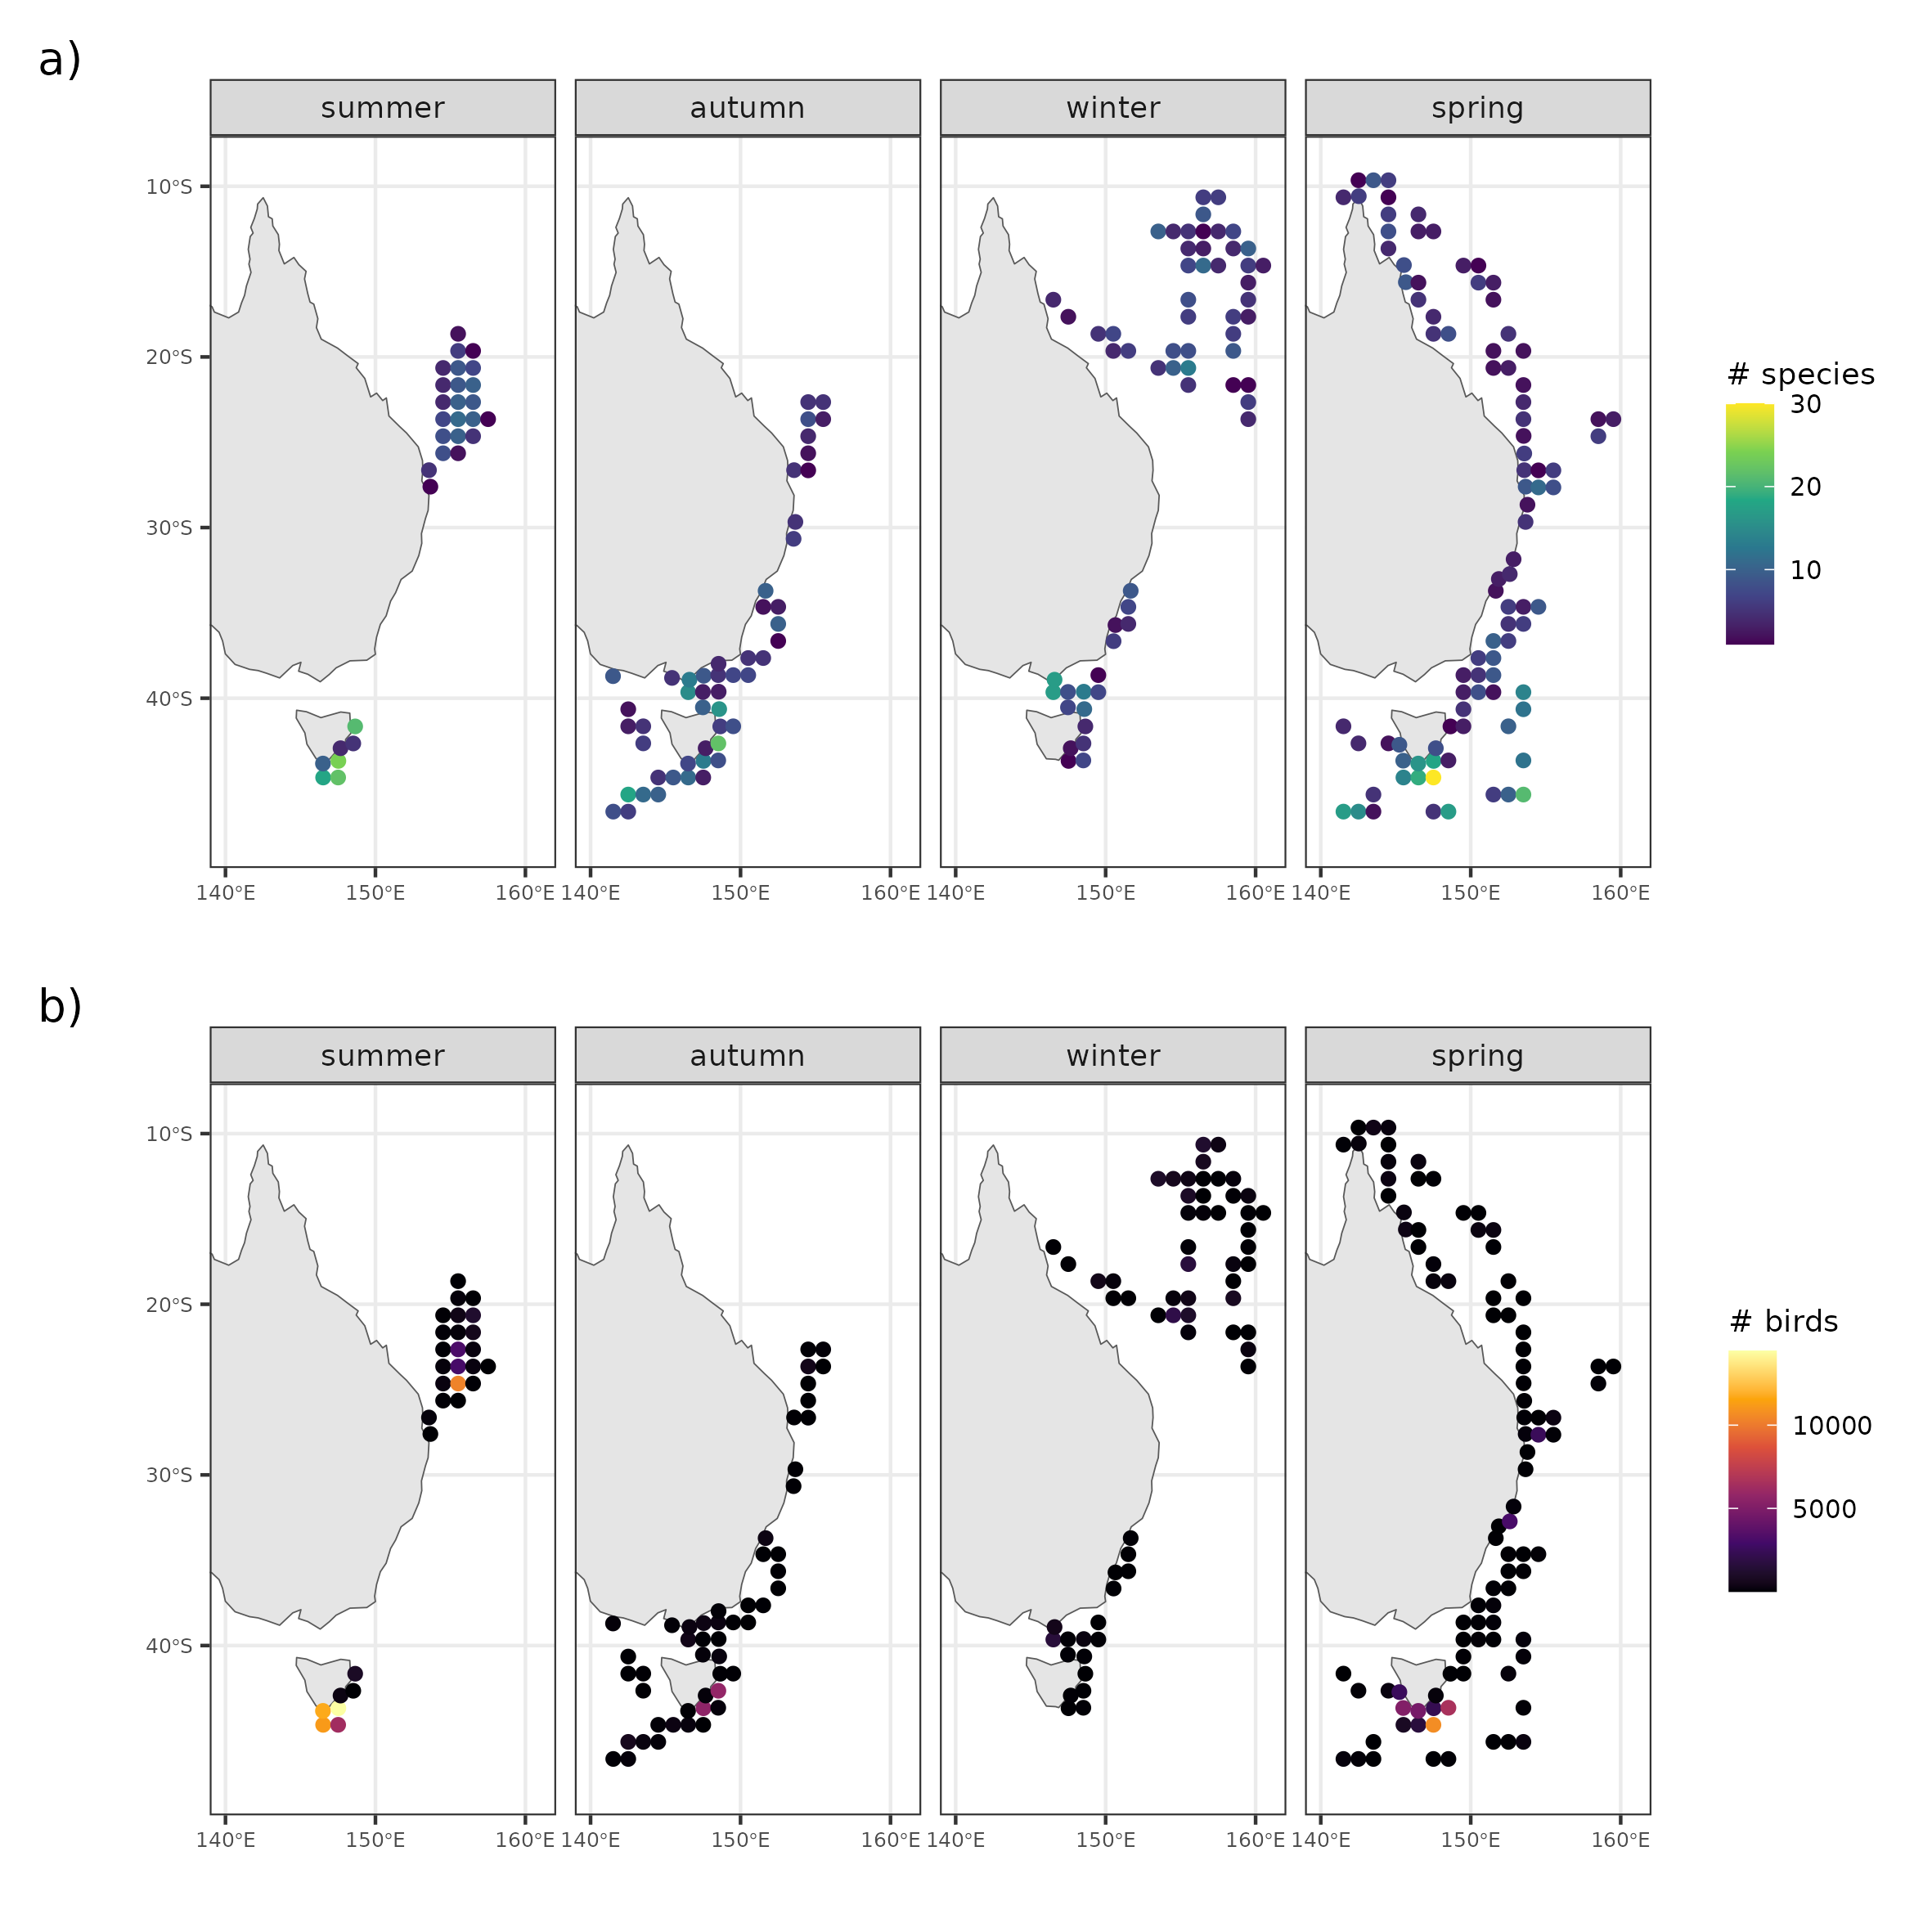
\includegraphics{../results/FigS2_map-effort-spp-richness-and-total-birds-seasons.png}
\caption{\textbf{Figure S2.} Species richness and the total number of
seabirds counted off eastern Australia during Australasian Seabird
Group's ship-based surveys between 2016--2021, by grid/season, after
data aggregation (see \emph{Methods} in the main text). Dots represent
the grid centroids.}
\end{figure}

\newpage

\begin{figure}
\centering
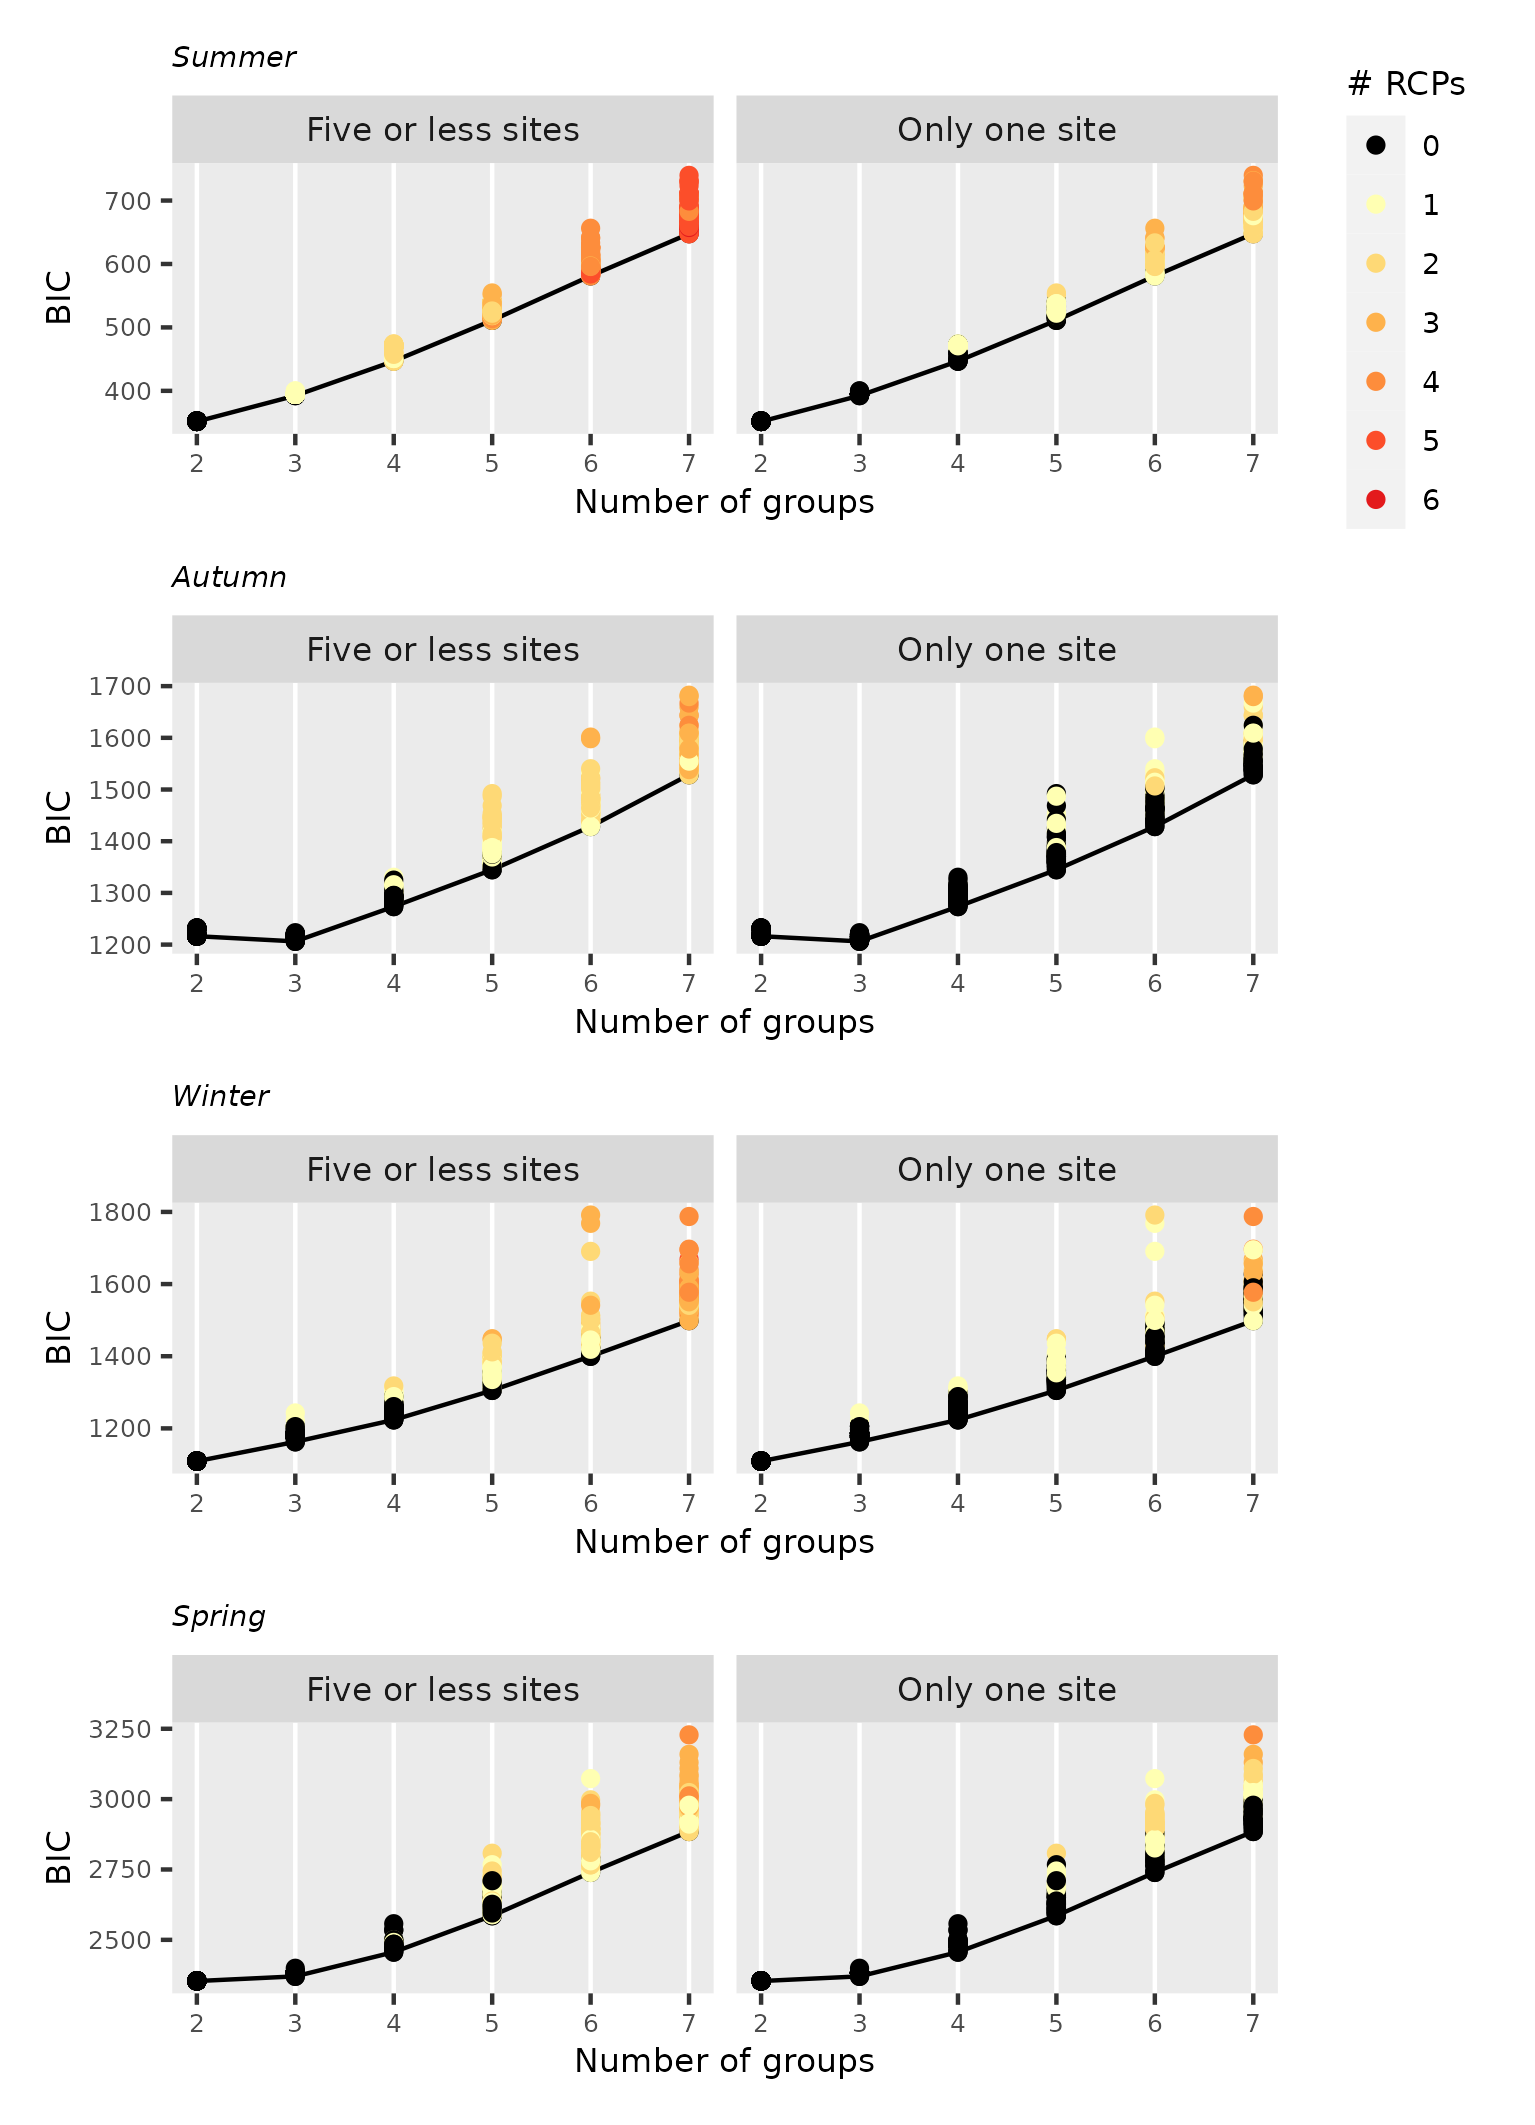
\includegraphics{../results/FigS3_1_multifit-Bernoulli.png}
\caption{\textbf{Figure S3.1.} Multifit plot for Region of Common
Profiles (RCP) for each seasonal presence-absence model, applied to
seabirds off eastern Australia. The number of groups with the lowest BIC
value indicates the best number of groups (assemblages) that describes
the data. For each number of groups, we ran 100 models with random
starting values to avoid getting stuck in an incorrect `optima' (see
\emph{Methods} in the main text). The resulting plot also shows how many
groups were `empty' (colour scale) with `five or less' or `only one'
sites assigned to an RCP, i.e.~the model was fit with, say, 5 groups,
but 3 of them had `five or less' or `only one' sites (grids) allocated
to an RCP.}
\end{figure}

\newpage

\begin{figure}
\centering
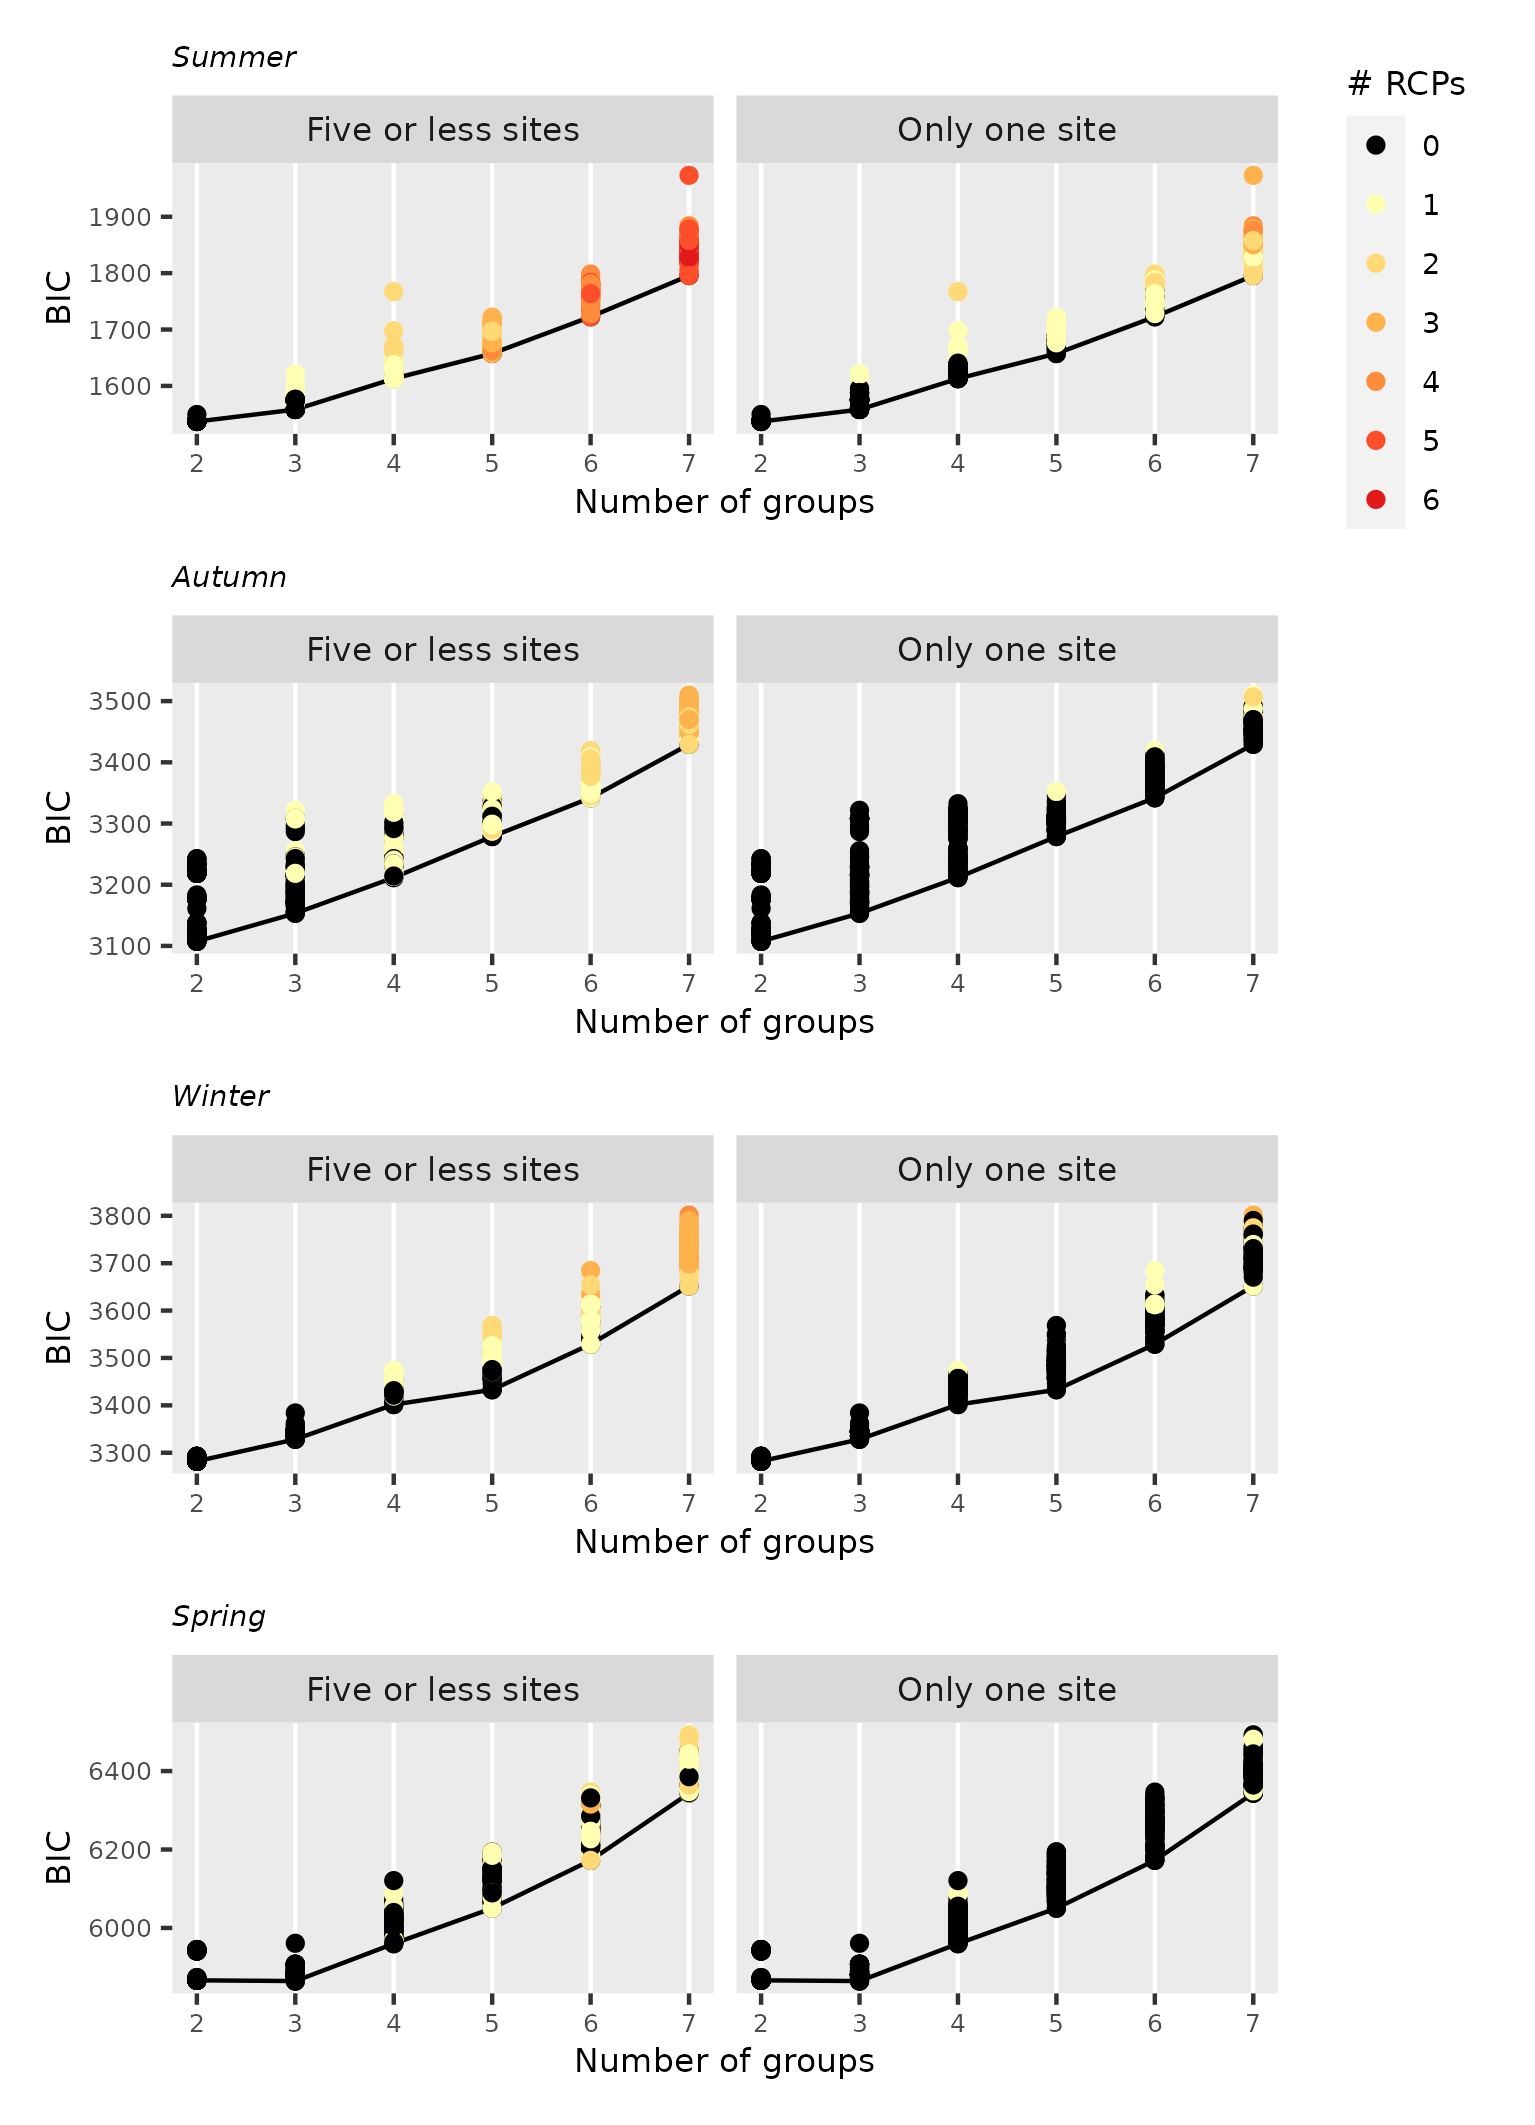
\includegraphics{../results/FigS3_2_multifit-NegBin.png}
\caption{\textbf{Figure S3.2.} Multifit plot for Region of Common
Profiles (RCP) for each seasonal abundance (count) model, applied to
seabirds off eastern Australia. The number of groups with the lowest BIC
value indicates the best number of groups (assemblages) that describes
the data. For each number of groups, we ran 100 models with random
starting values to avoid getting stuck in an incorrect `optima' (see
\emph{Methods} in the main text). The resulting plot also shows how many
groups were `empty' (colour scale) with `five or less' or `only one'
sites assigned to an RCP, i.e.~the model was fit with, say, 5 groups,
but 3 of them had `five or less' or `only one' sites (grids) allocated
to an RCP.}
\end{figure}

\newpage

\begin{figure}
\centering
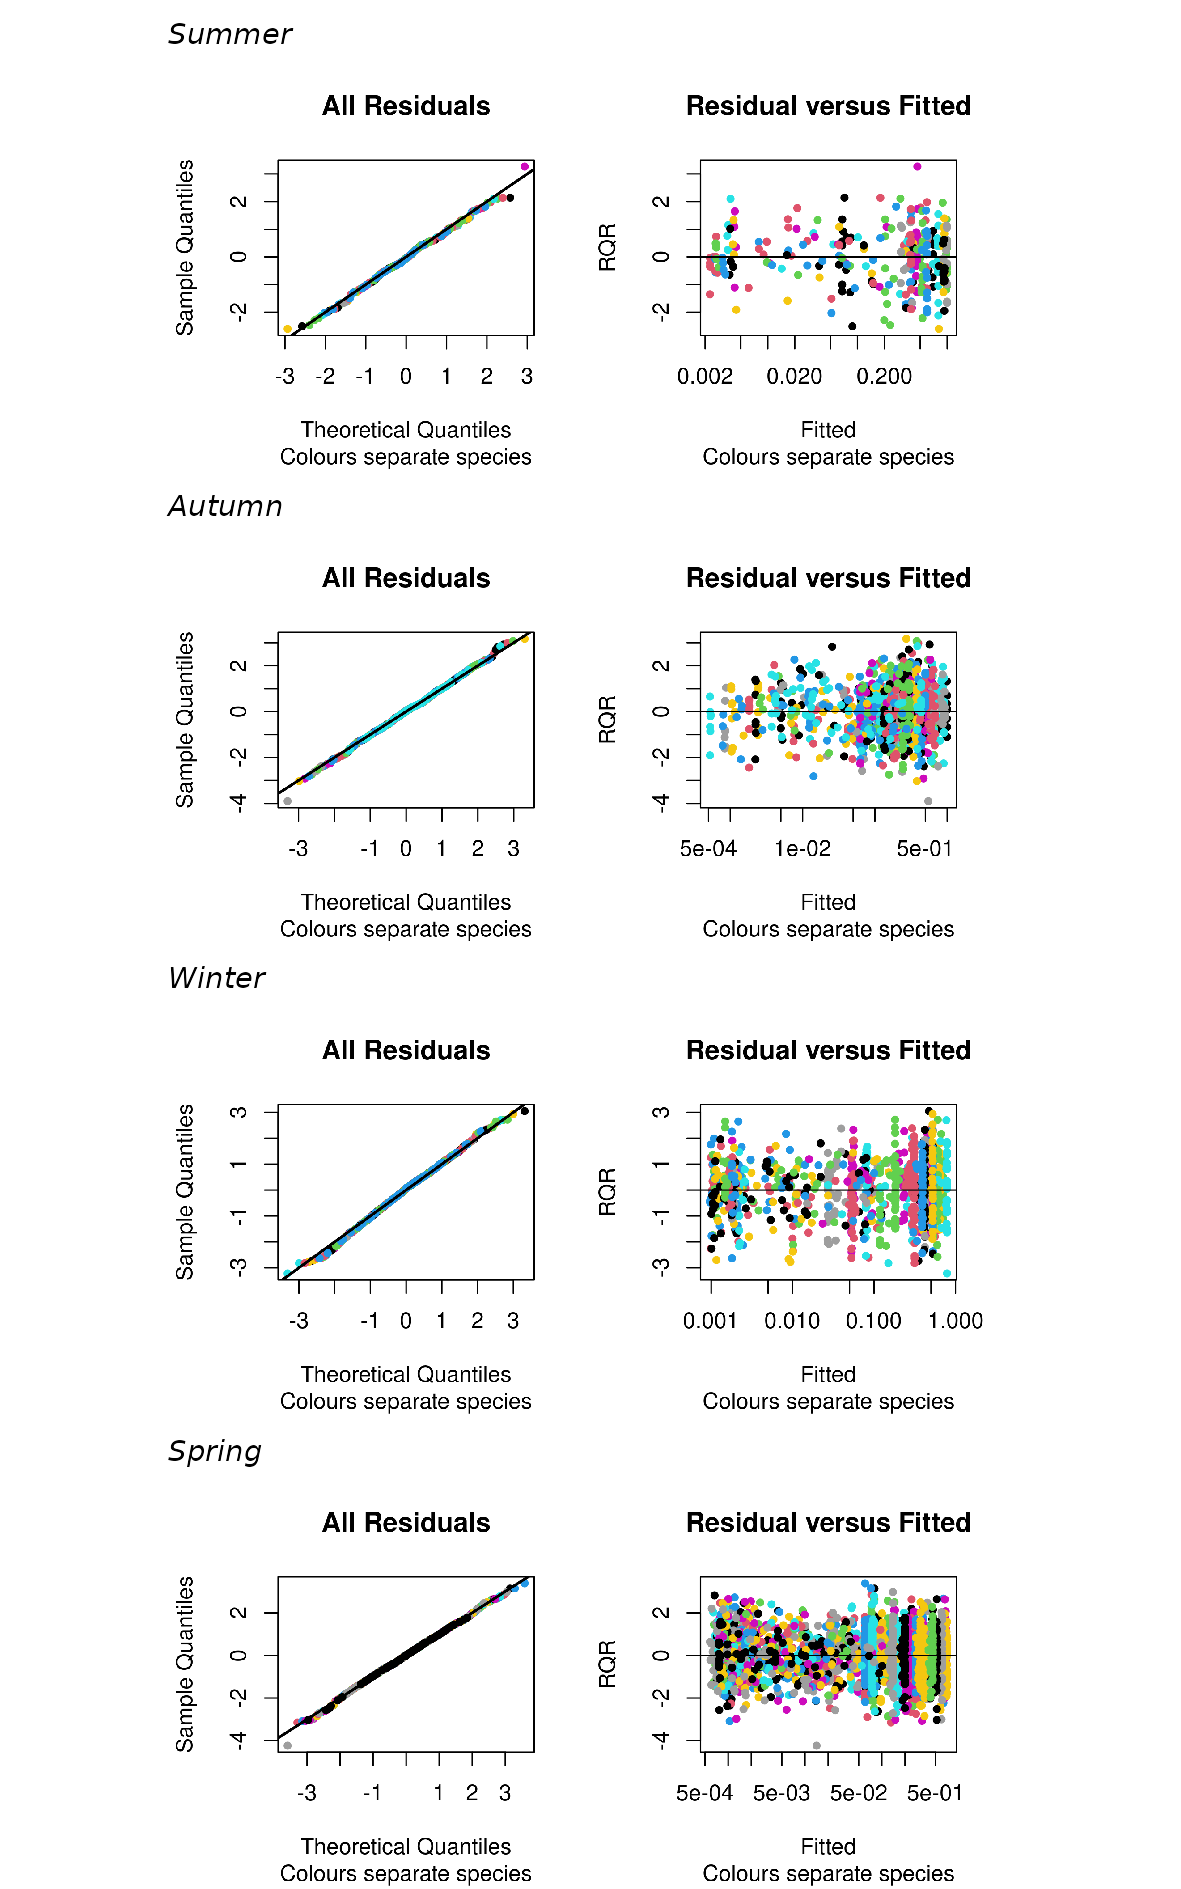
\includegraphics{../results/FigS4_1_best-model-residuals-Bernoulli.png}
\caption{\textbf{Figure S4.1.} Best model residuals for each seasonal
presence-absence Region of Common Profile model, applied to seabirds off
eastern Australia.}
\end{figure}

\newpage

\begin{figure}
\centering
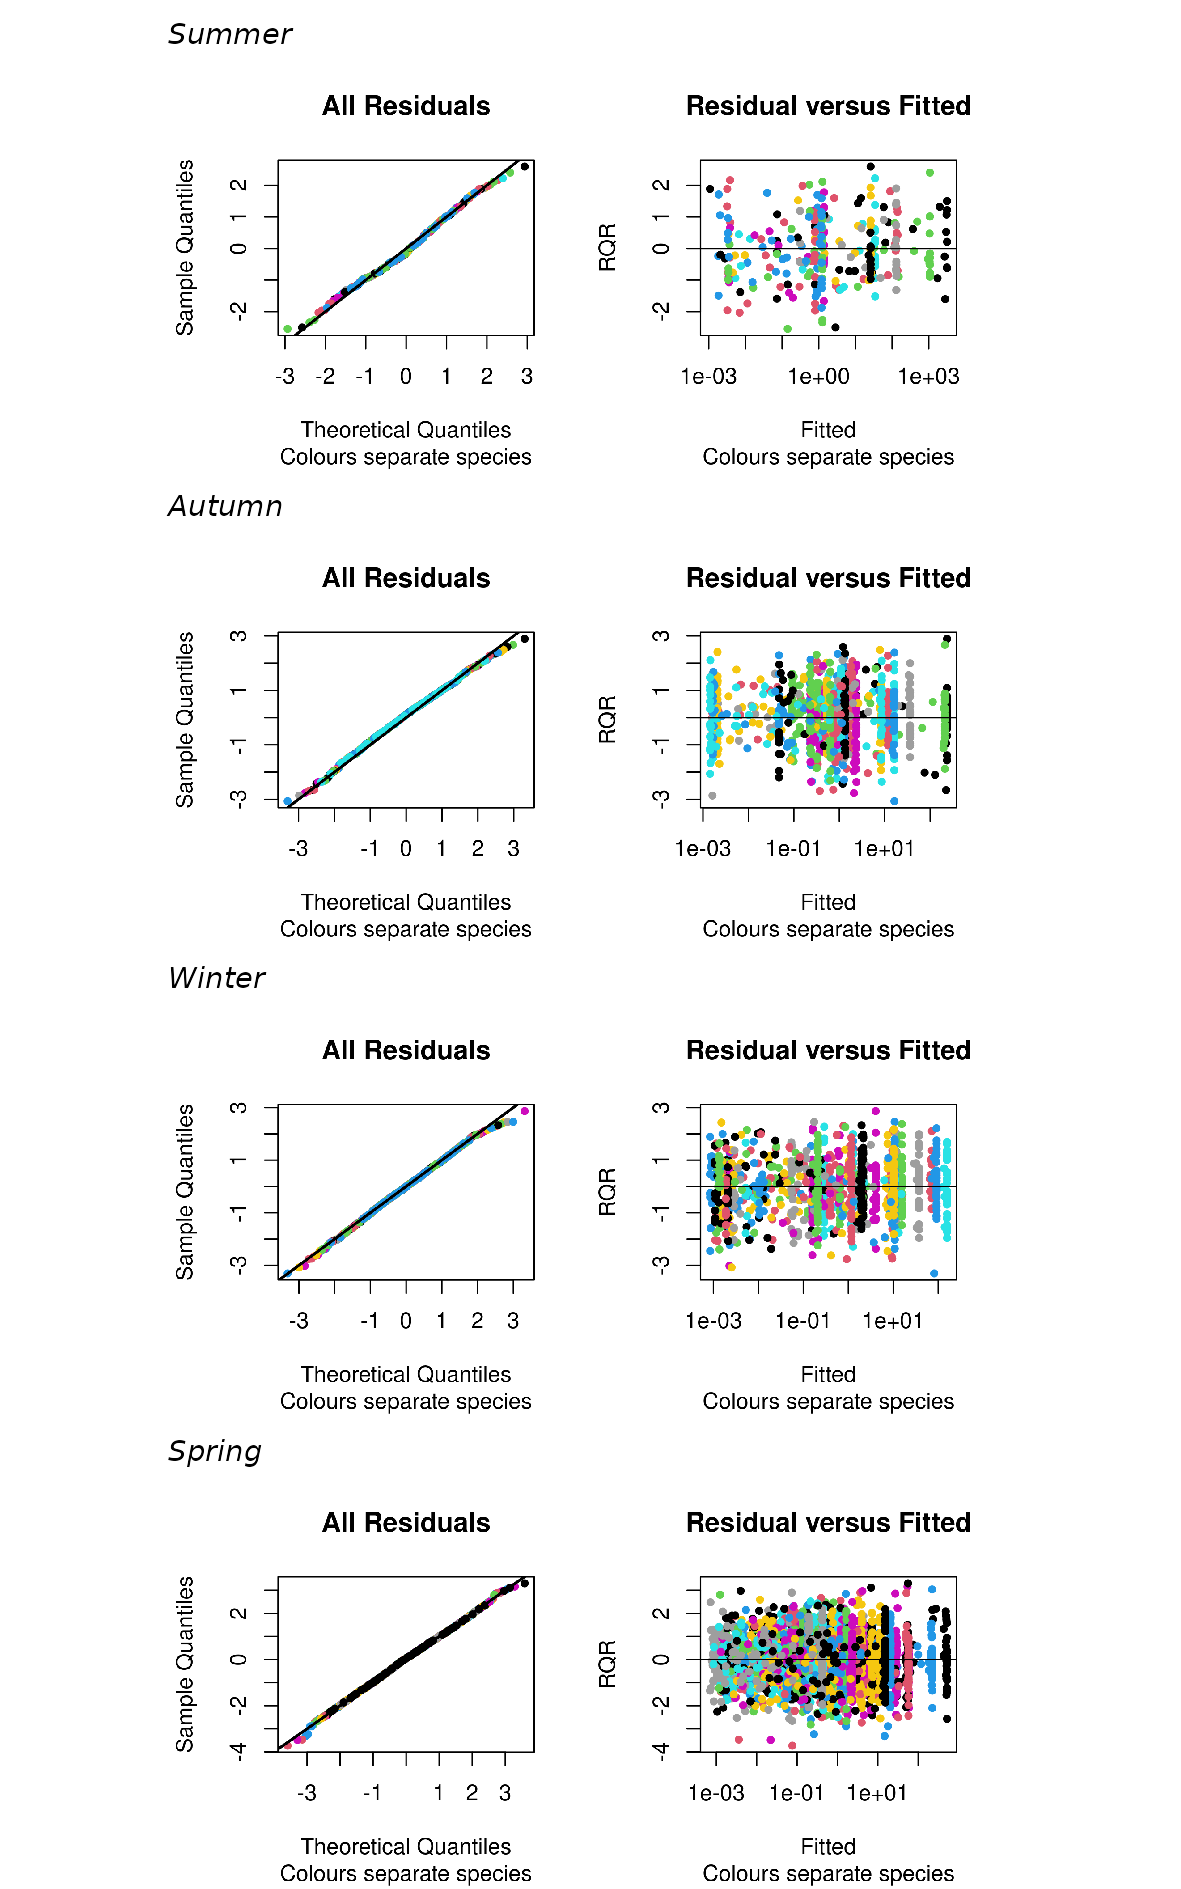
\includegraphics{../results/FigS4_2_best-model-residuals-NegBin.png}
\caption{\textbf{Figure S4.2.} Best model residuals for each seasonal
abundance (count) Region of Common Profile model, applied to seabirds
off eastern Australia.}
\end{figure}

\newpage

\begin{figure}
\centering
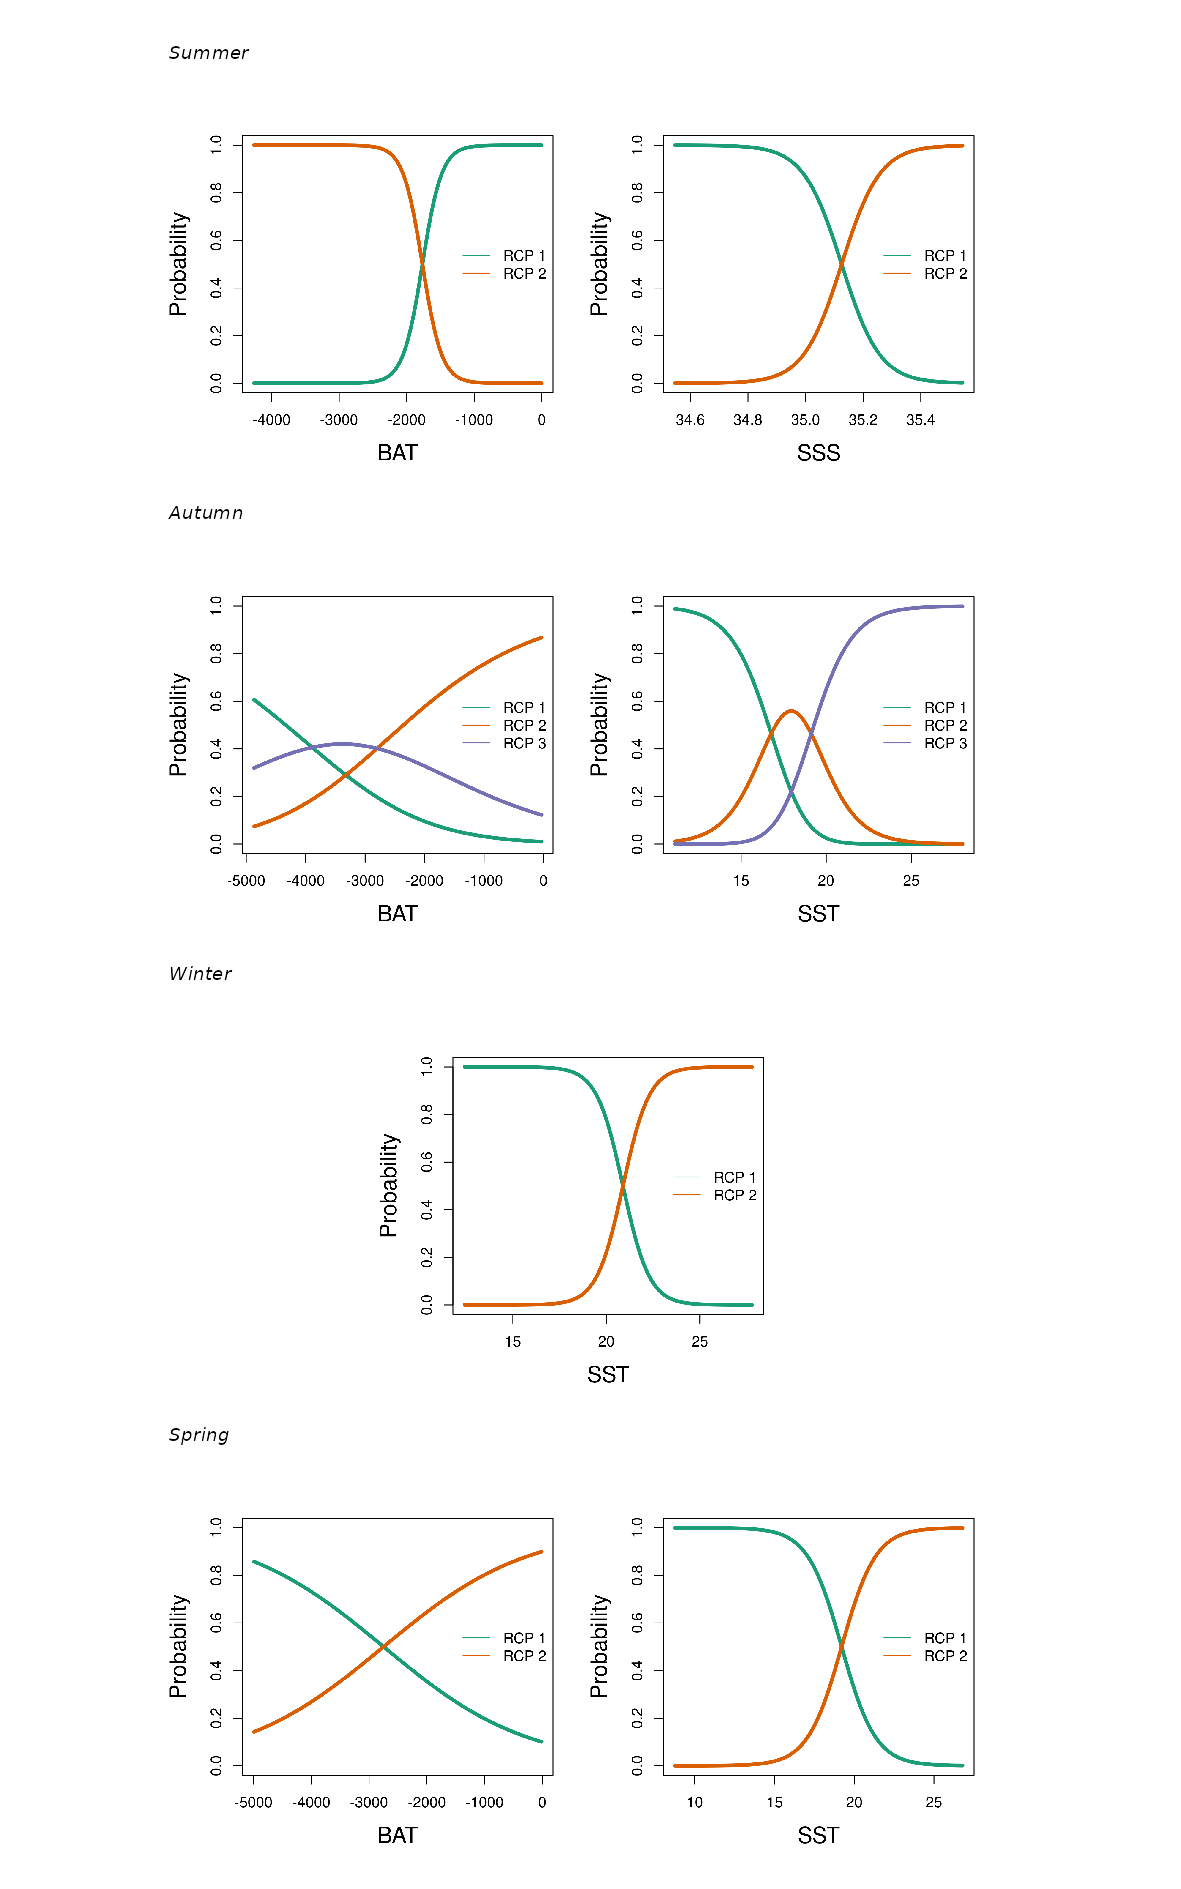
\includegraphics{../results/FigS6_1_partial-plots-Bernoulli.png}
\caption{\textbf{Figure S5.1.} Partial plots for the retained covariates
in the best seasonal models based on presence-absence data. The plot
shows the probability of belonging to a Region of Common Profiles (RCP)
against the environmental value. Refer to Table 1 in the main text for
the environmental data acronyms.}
\end{figure}

\newpage

\begin{landscape}

\begin{figure}
\centering
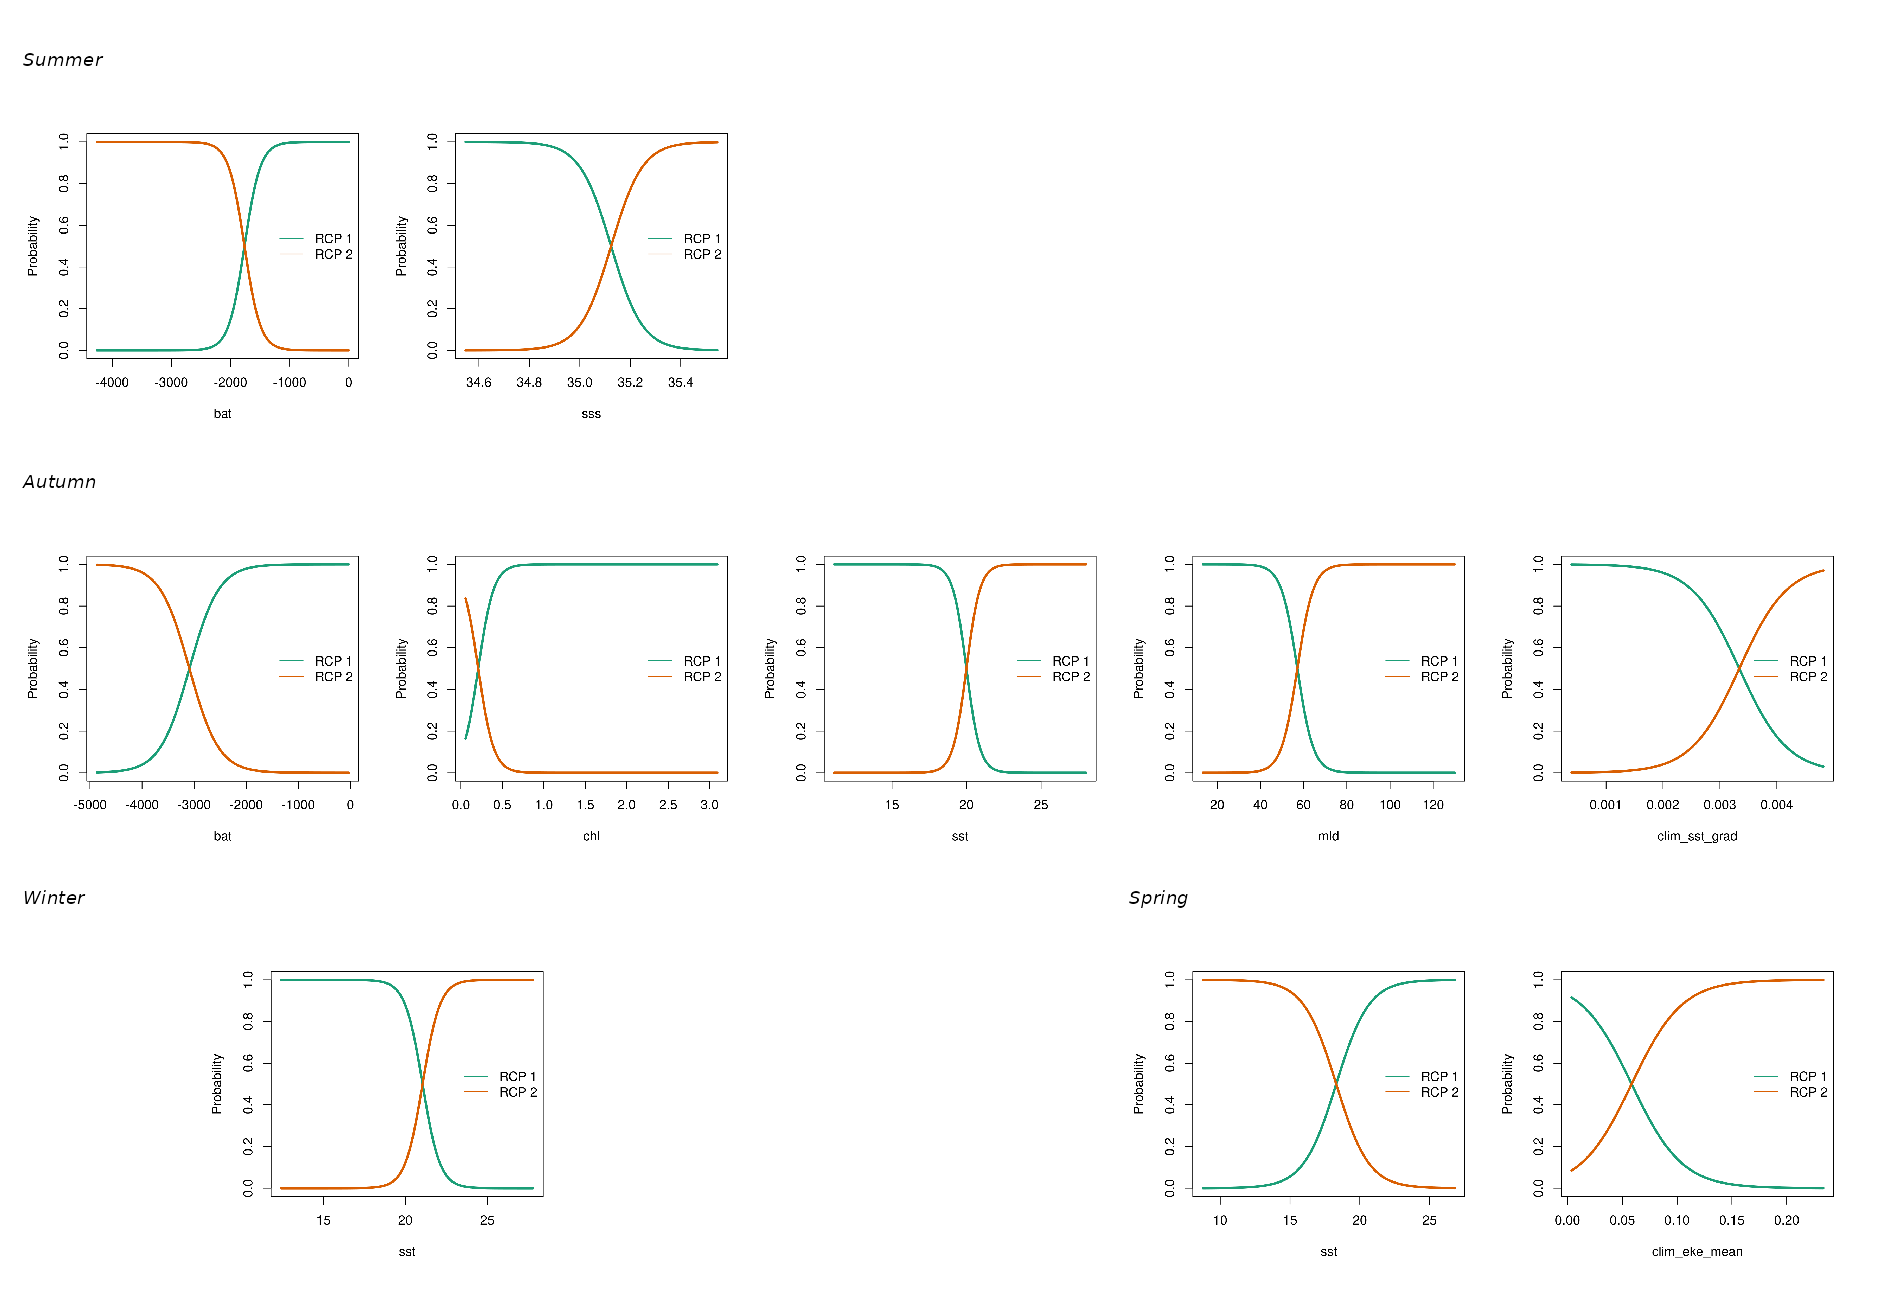
\includegraphics{../results/FigS6_2_partial-plots-NegBin.png}
\caption{\textbf{Figure S5.2.} Partial plots for the retained covariates
in the best seasonal models based on abundance data. The plot shows the
probability of belonging to a Region of Common Profiles (RCP) against
the environmental value. Refer to Table 1 in the main text for the
environmental data acronyms.}
\end{figure}

\newpage

\begin{figure}
\centering
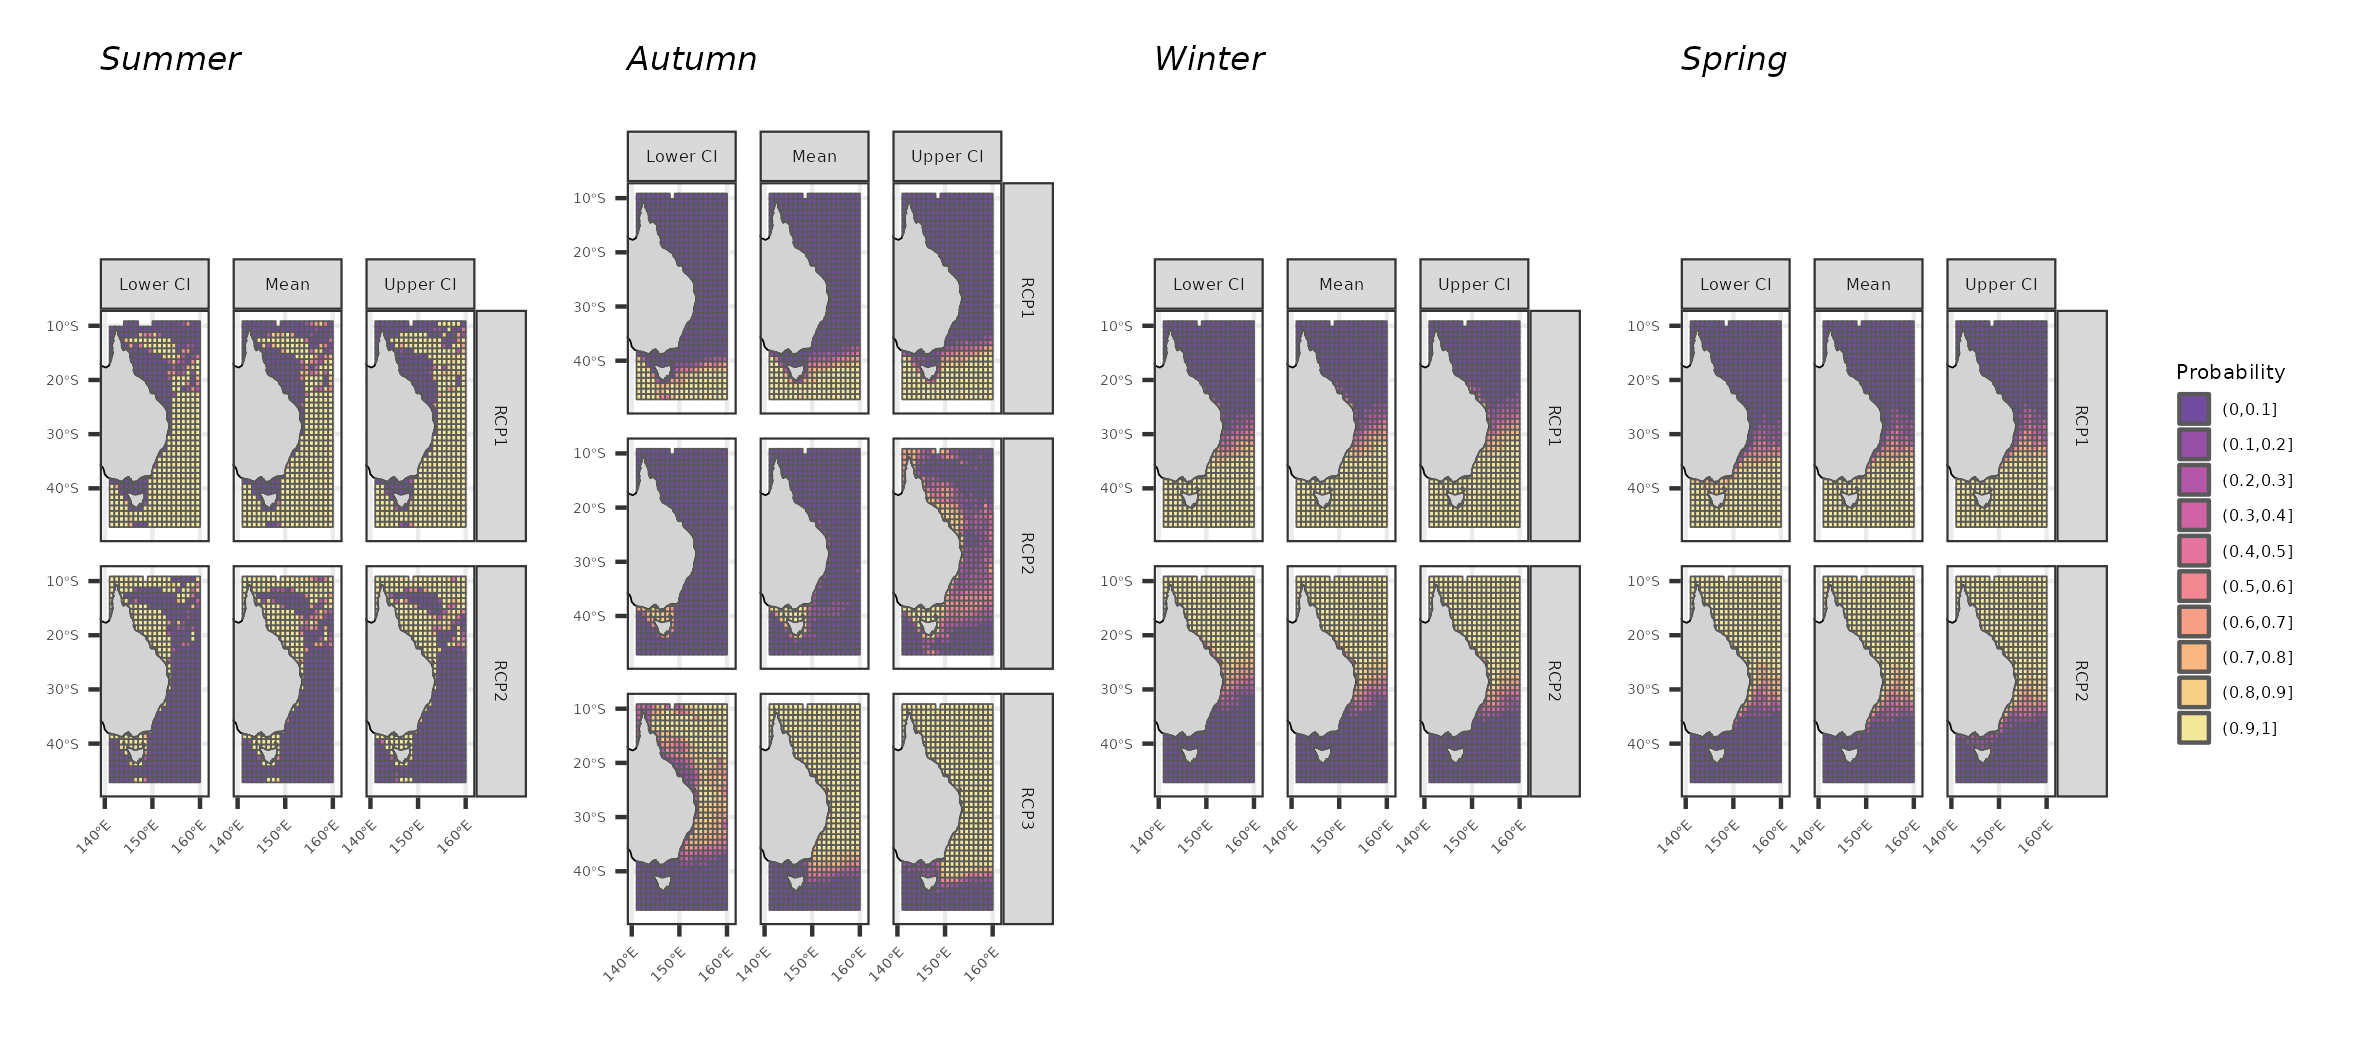
\includegraphics{../results/FigS5_1_prob-pred-Bernoulli.png}
\caption{\textbf{Figure S6.1.} Predicted probability membership of for
each seabird assemblage (Region of Common Profiles; RCP) and grid, off
eastern Australia, from presence-absence models. The central column,
`mean', corresponds to the point prediction and Bayesian bootstraped,
lower and upper confidence intervals (CI), on its sides.}
\end{figure}

\newpage

\begin{figure}
\centering
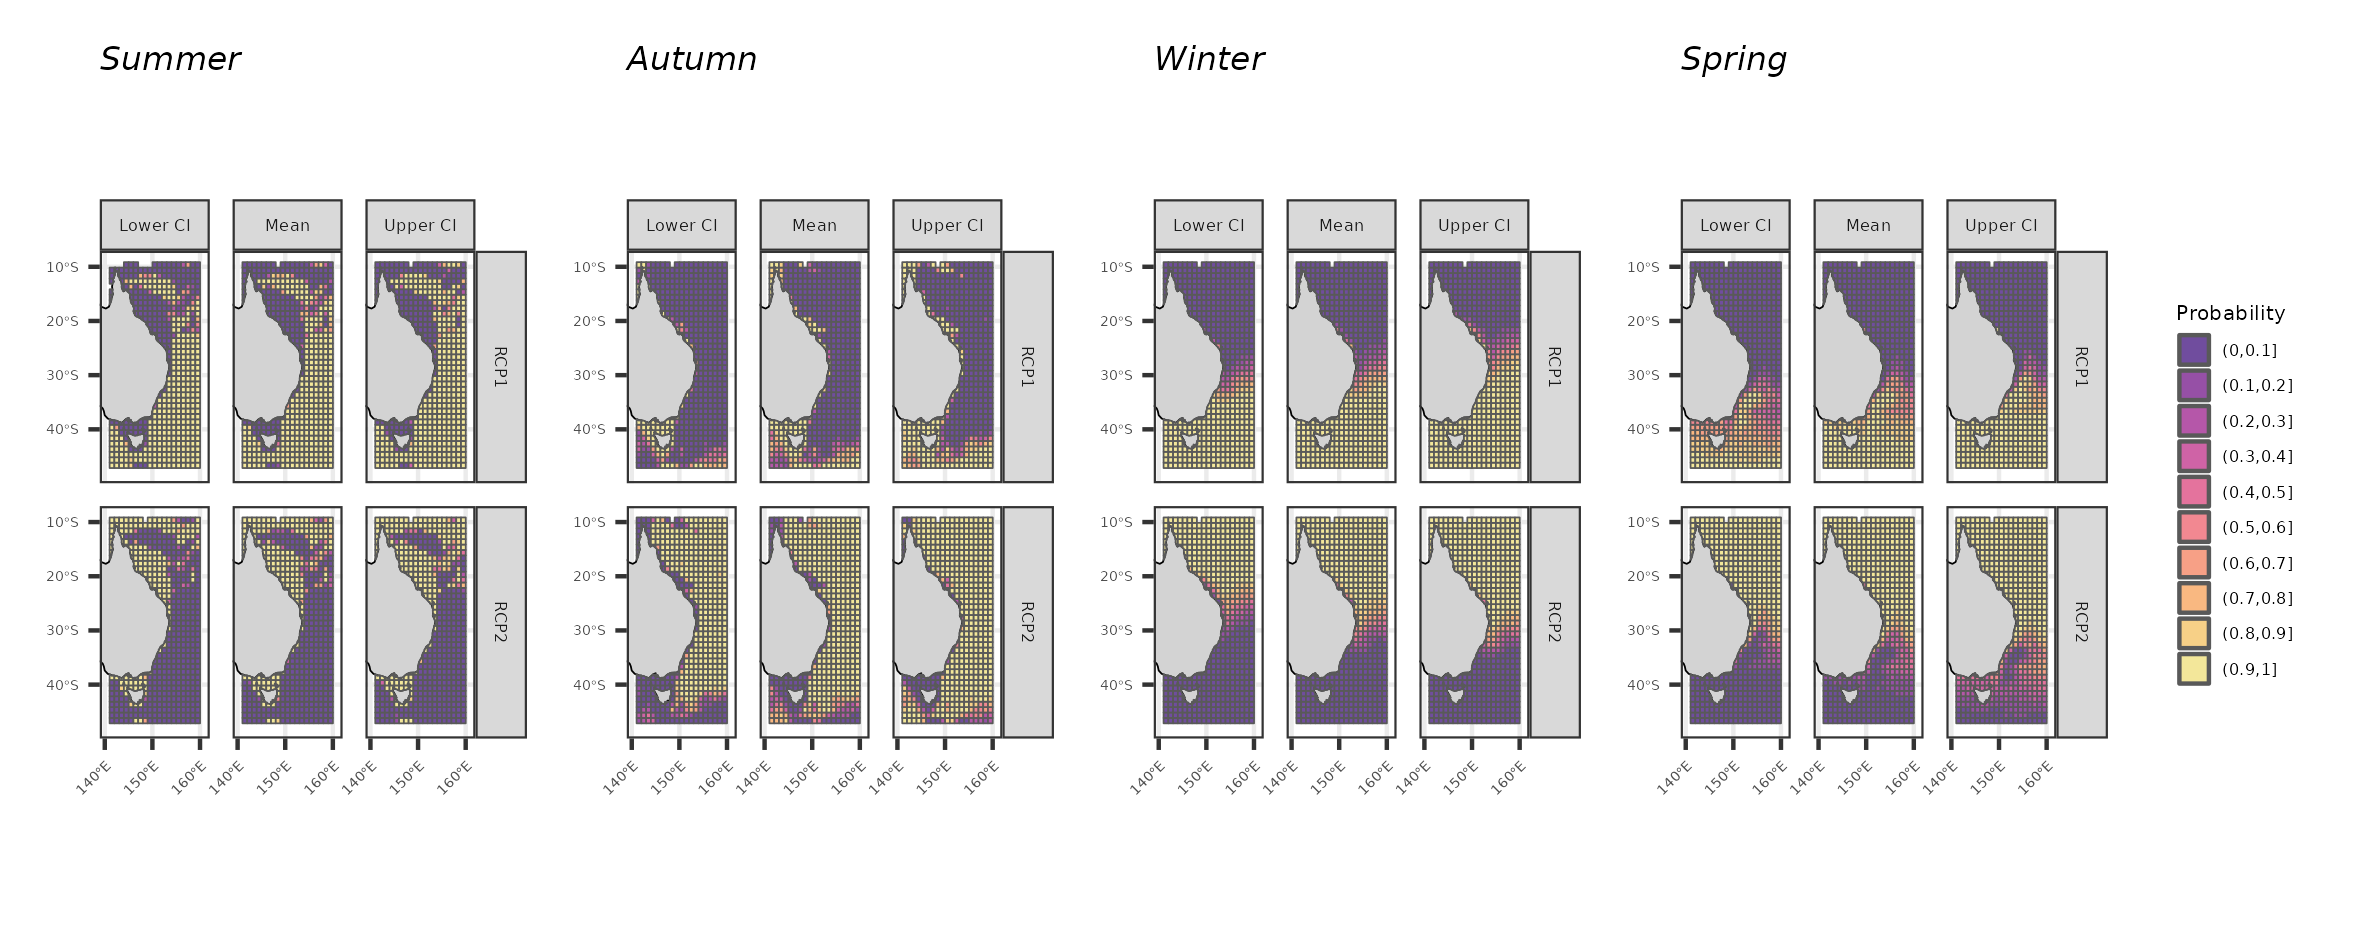
\includegraphics{../results/FigS5_2_prob-pred-NegBin.png}
\caption{\textbf{Figure S6.2.} Predicted probability membership of for
each seabird assemblage (Region of Common Profiles; RCP) and grid, off
eastern Australia, from abundance (count) models. The central column,
`mean', corresponds to the point prediction and Bayesian bootstraped,
lower and upper confidence intervals (CI), on its sides.}
\end{figure}

\newpage

\begin{figure}
\centering
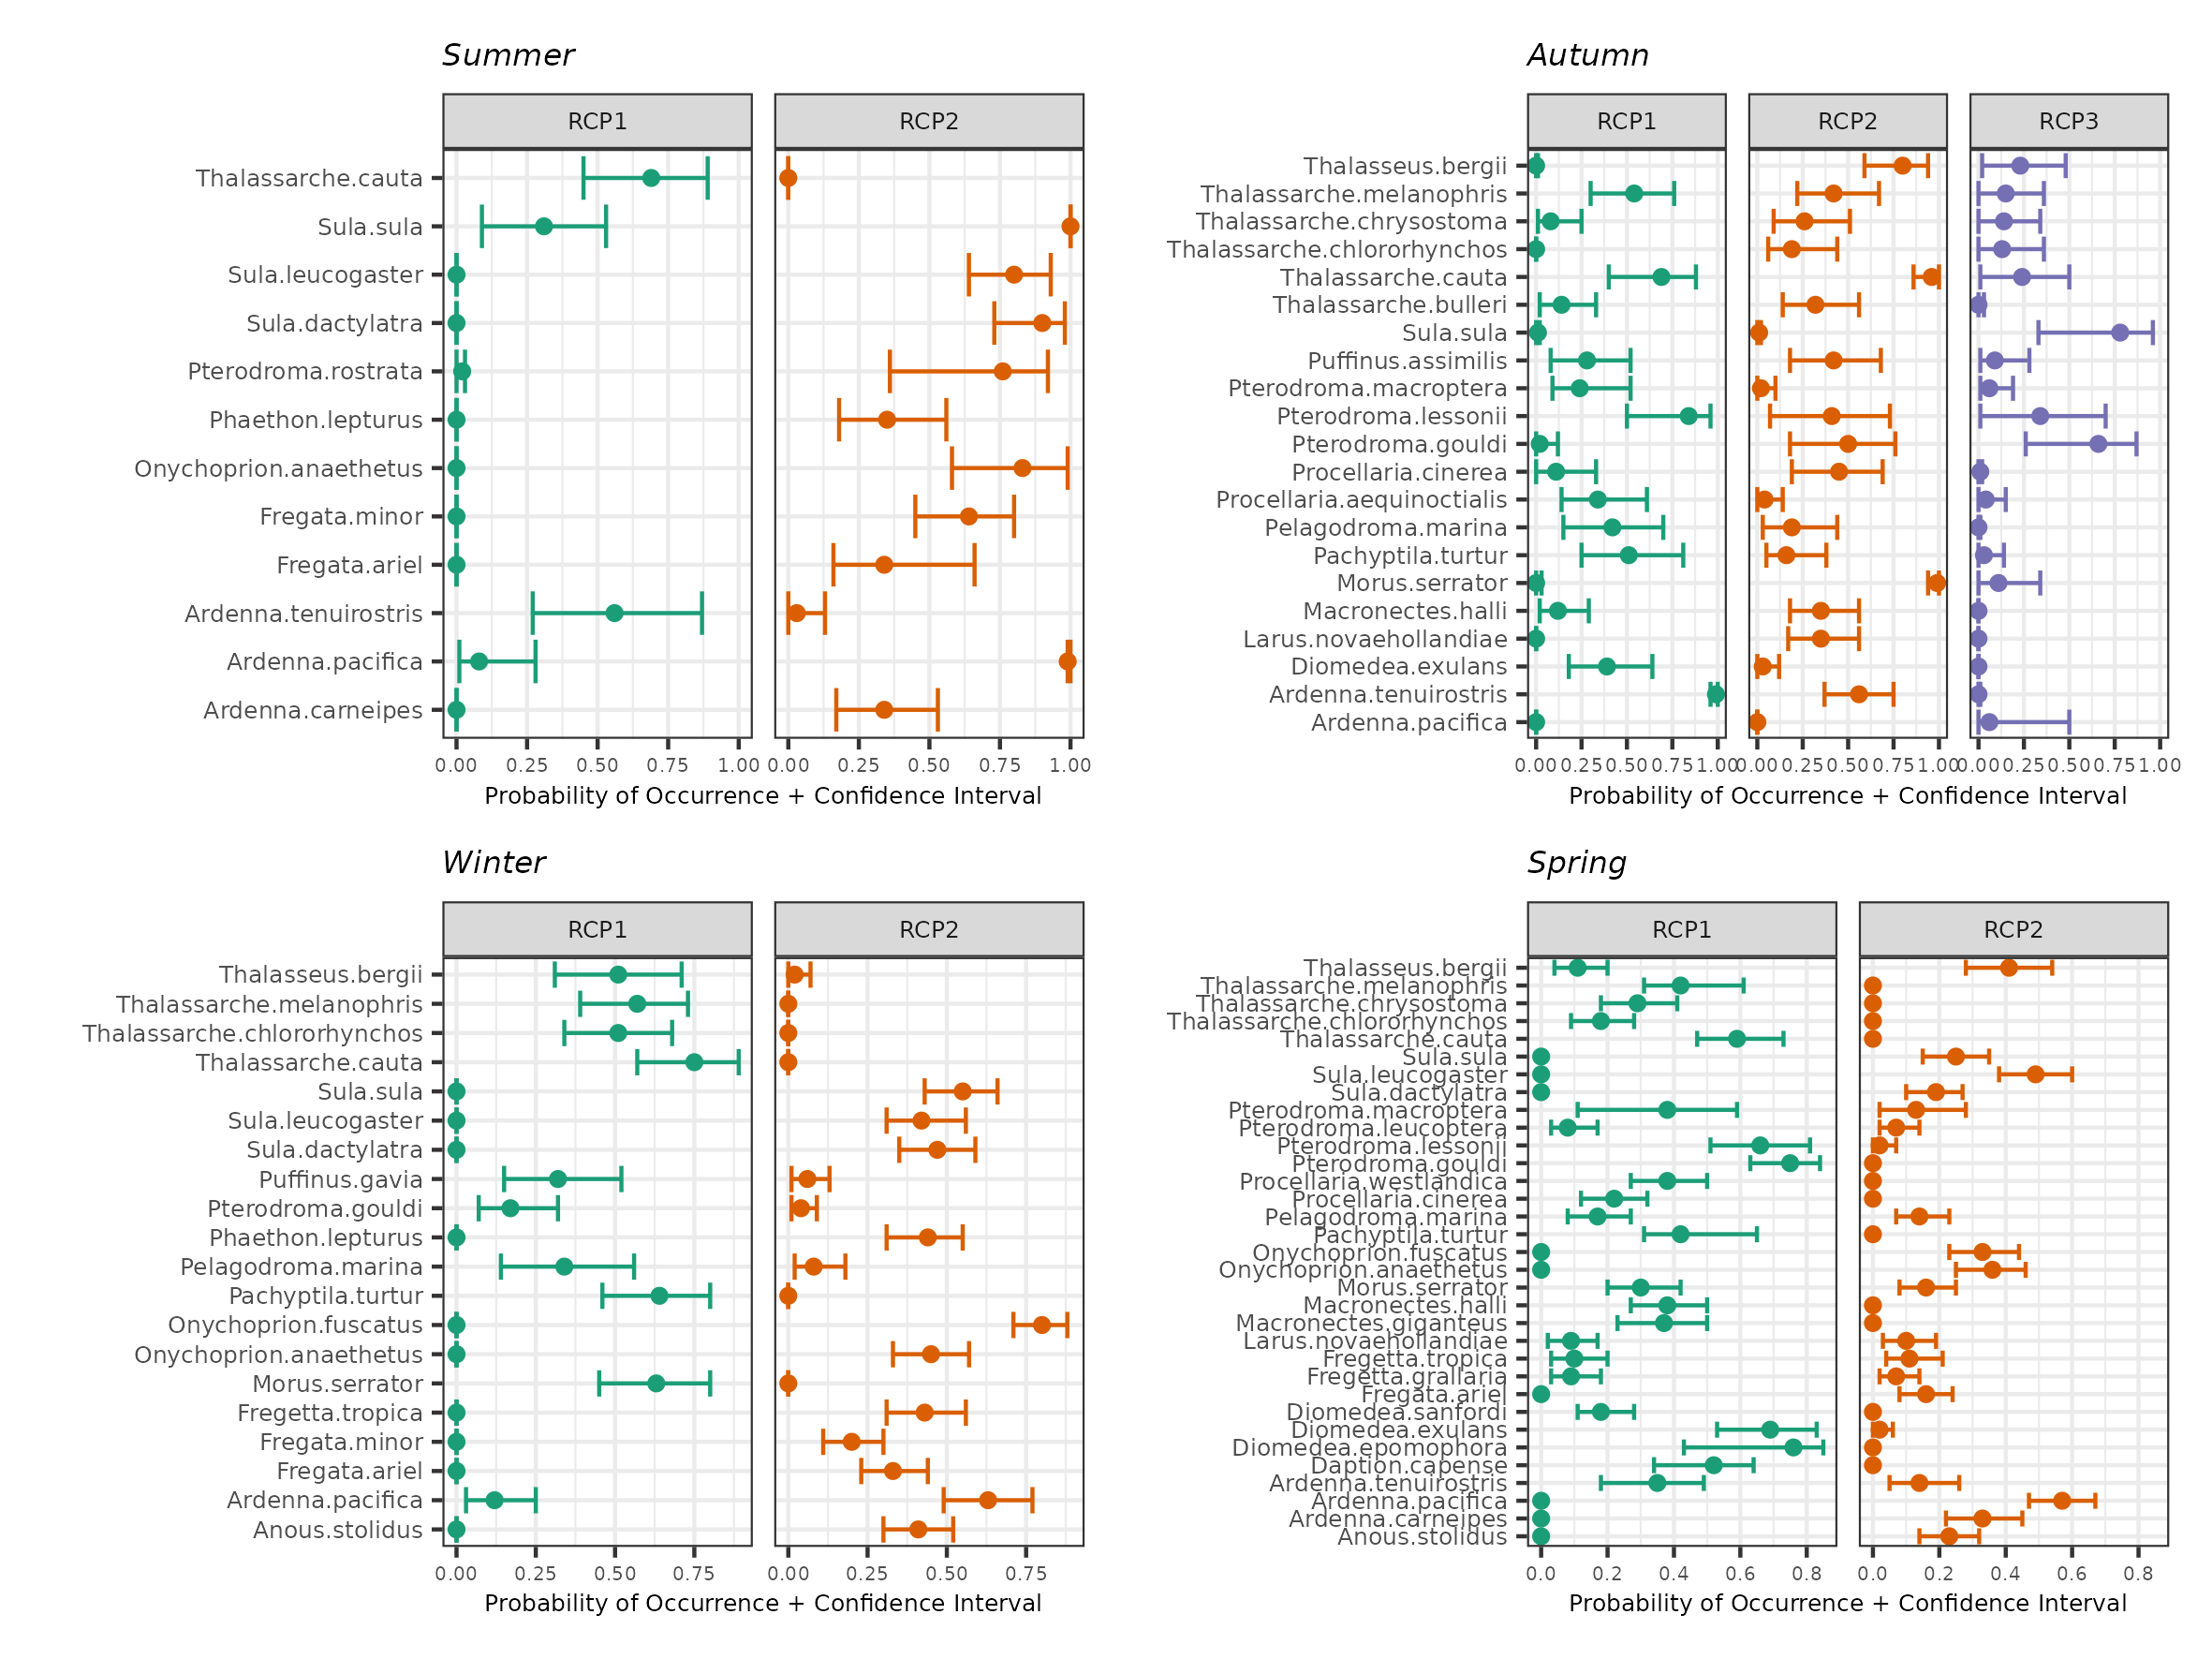
\includegraphics{../results/FigS7_1_spp-profiles-Bernoulli.png}
\caption{\textbf{Figure S7.1.} Species profiles for each assemblage
(Region of Common Profiles; RCP) for each seasonal presence-absence
model. Values are the average and confidence intervals of probability of
occurrence for each species, based on 1000 Bayesian bootstraps.}
\end{figure}

\newpage

\begin{figure}
\centering
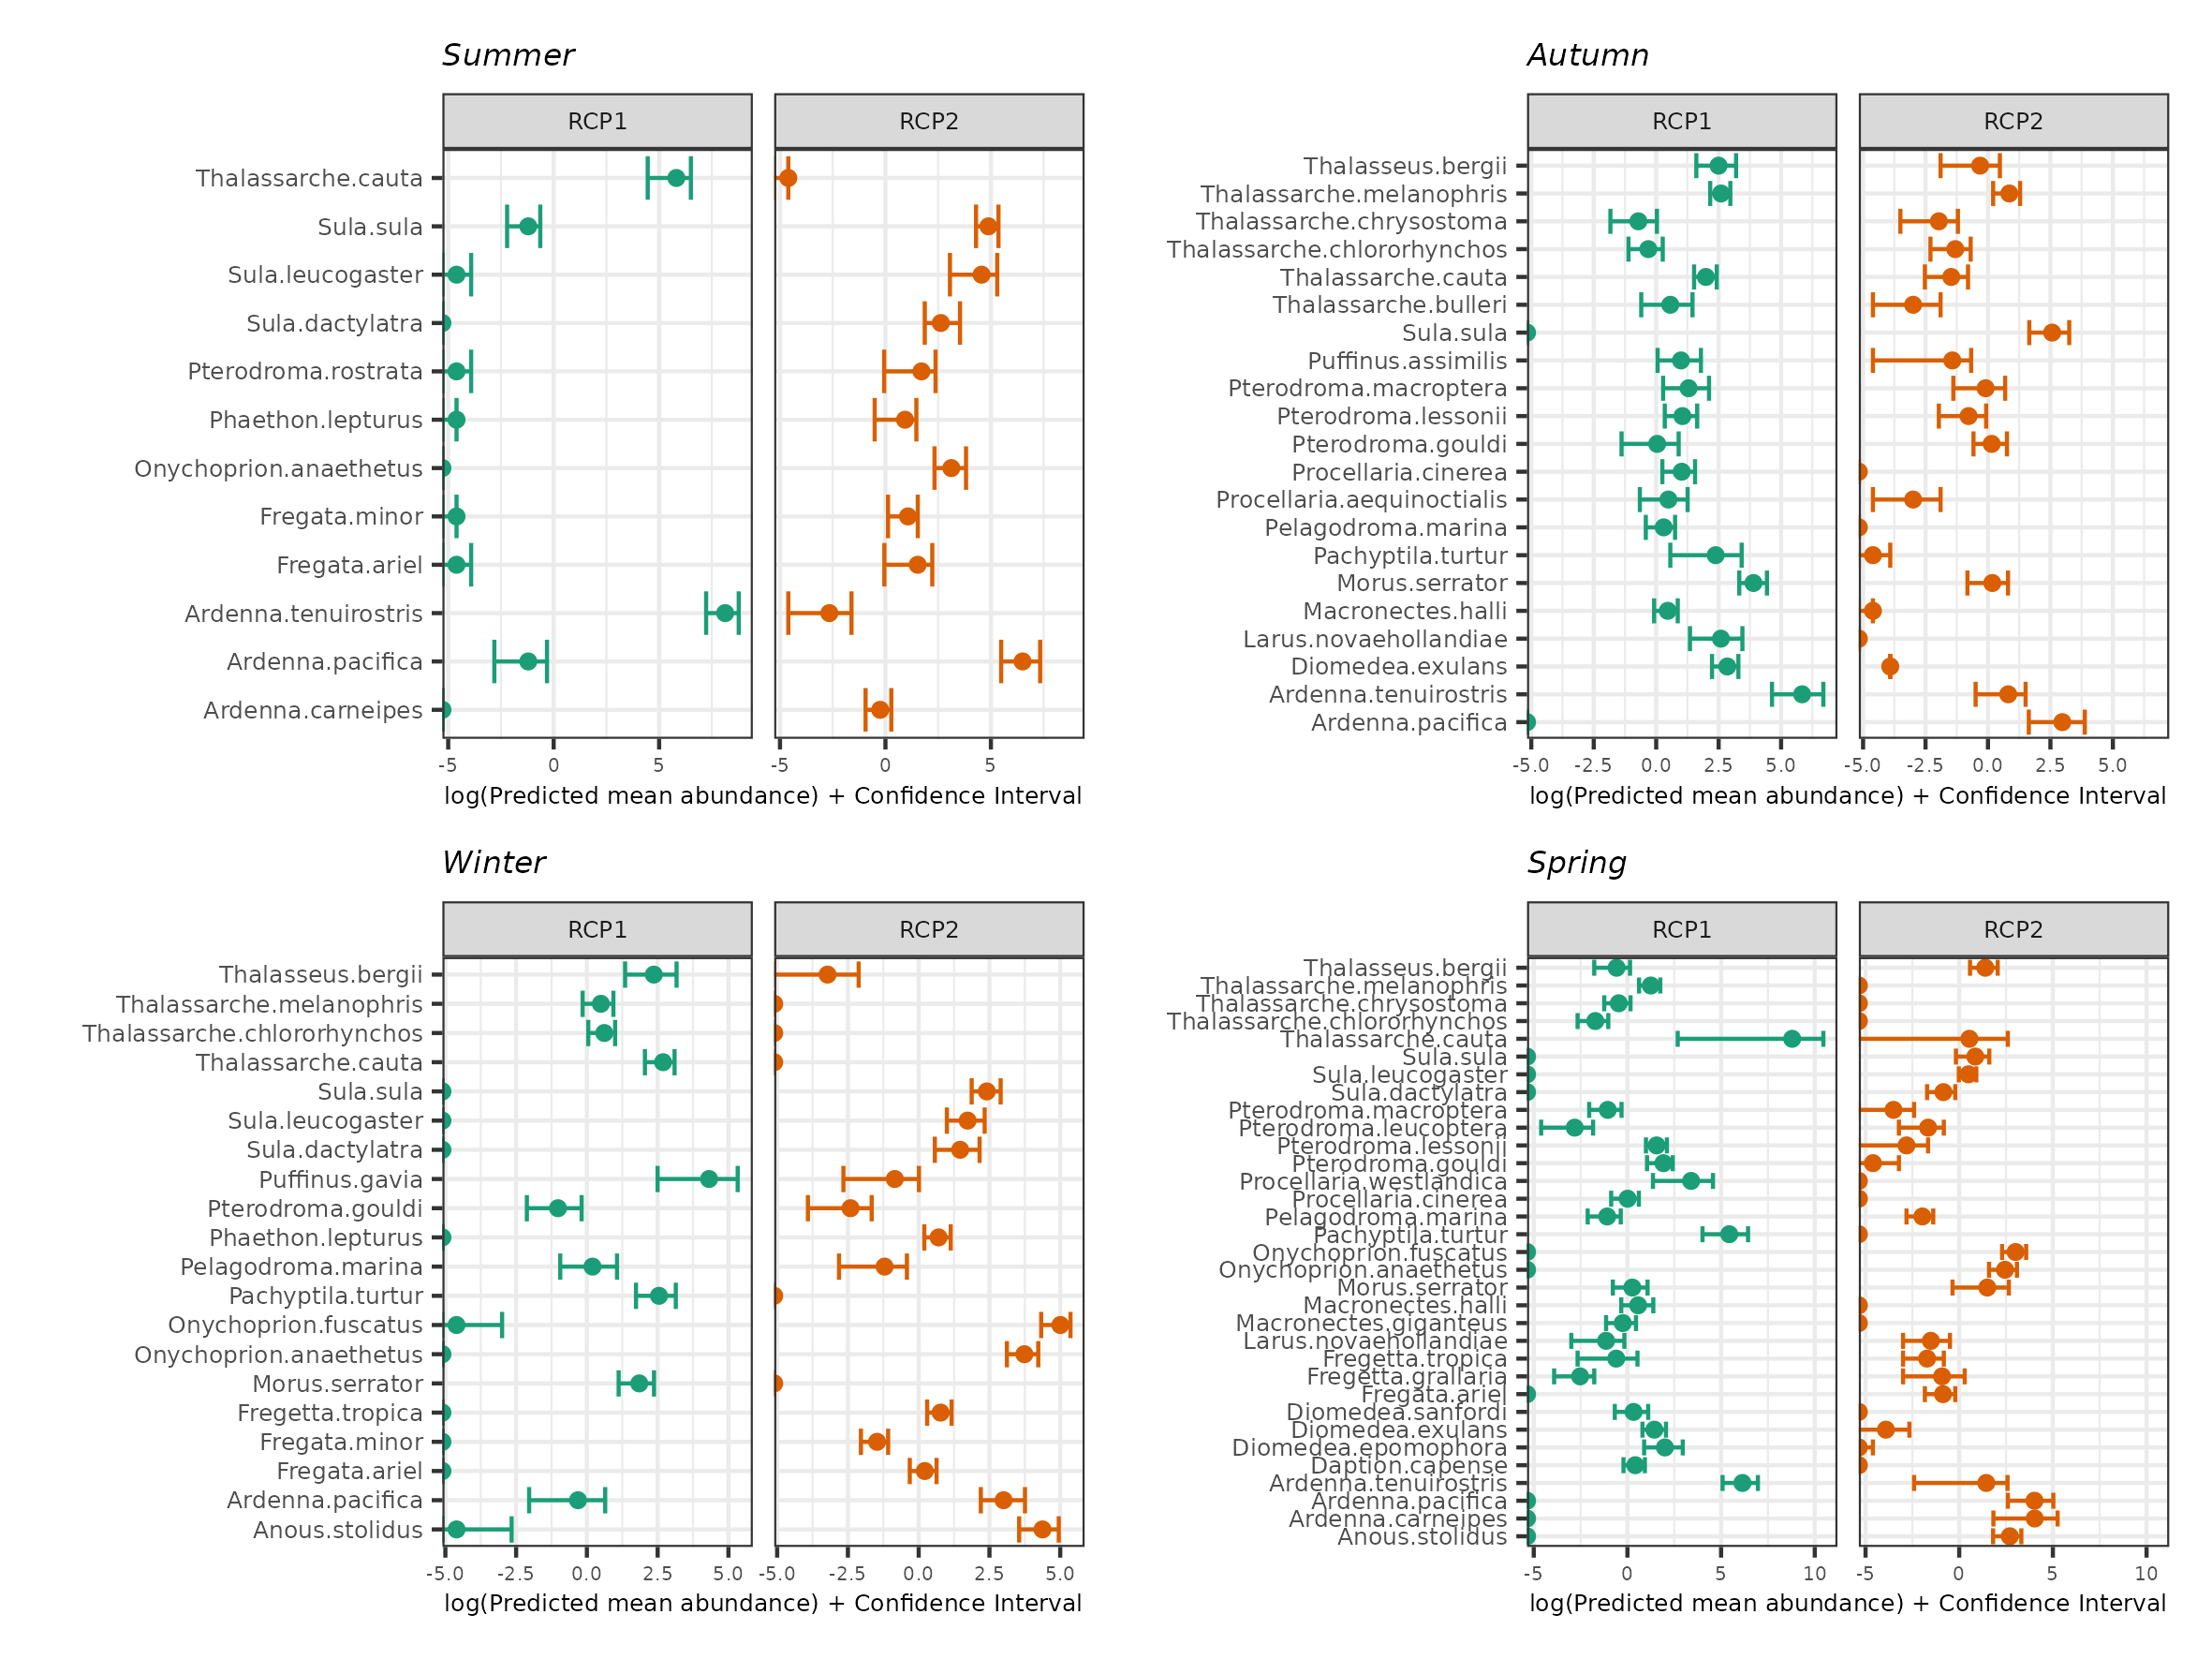
\includegraphics{../results/FigS7_2_spp-profiles-NegBin.png}
\caption{\textbf{Figure S7.2.} Species profiles for each assemblage
(Region of Common Profiles; RCP) for each seasonal abundance (count)
model. Values are the average and confidence intervals of predicted mean
abundance for each species, based on 1000 Bayesian bootstraps. Values
were log10-transformed to accommodate the high variation between
species.}
\end{figure}

\end{landscape}

\newpage

\begin{figure}
\centering
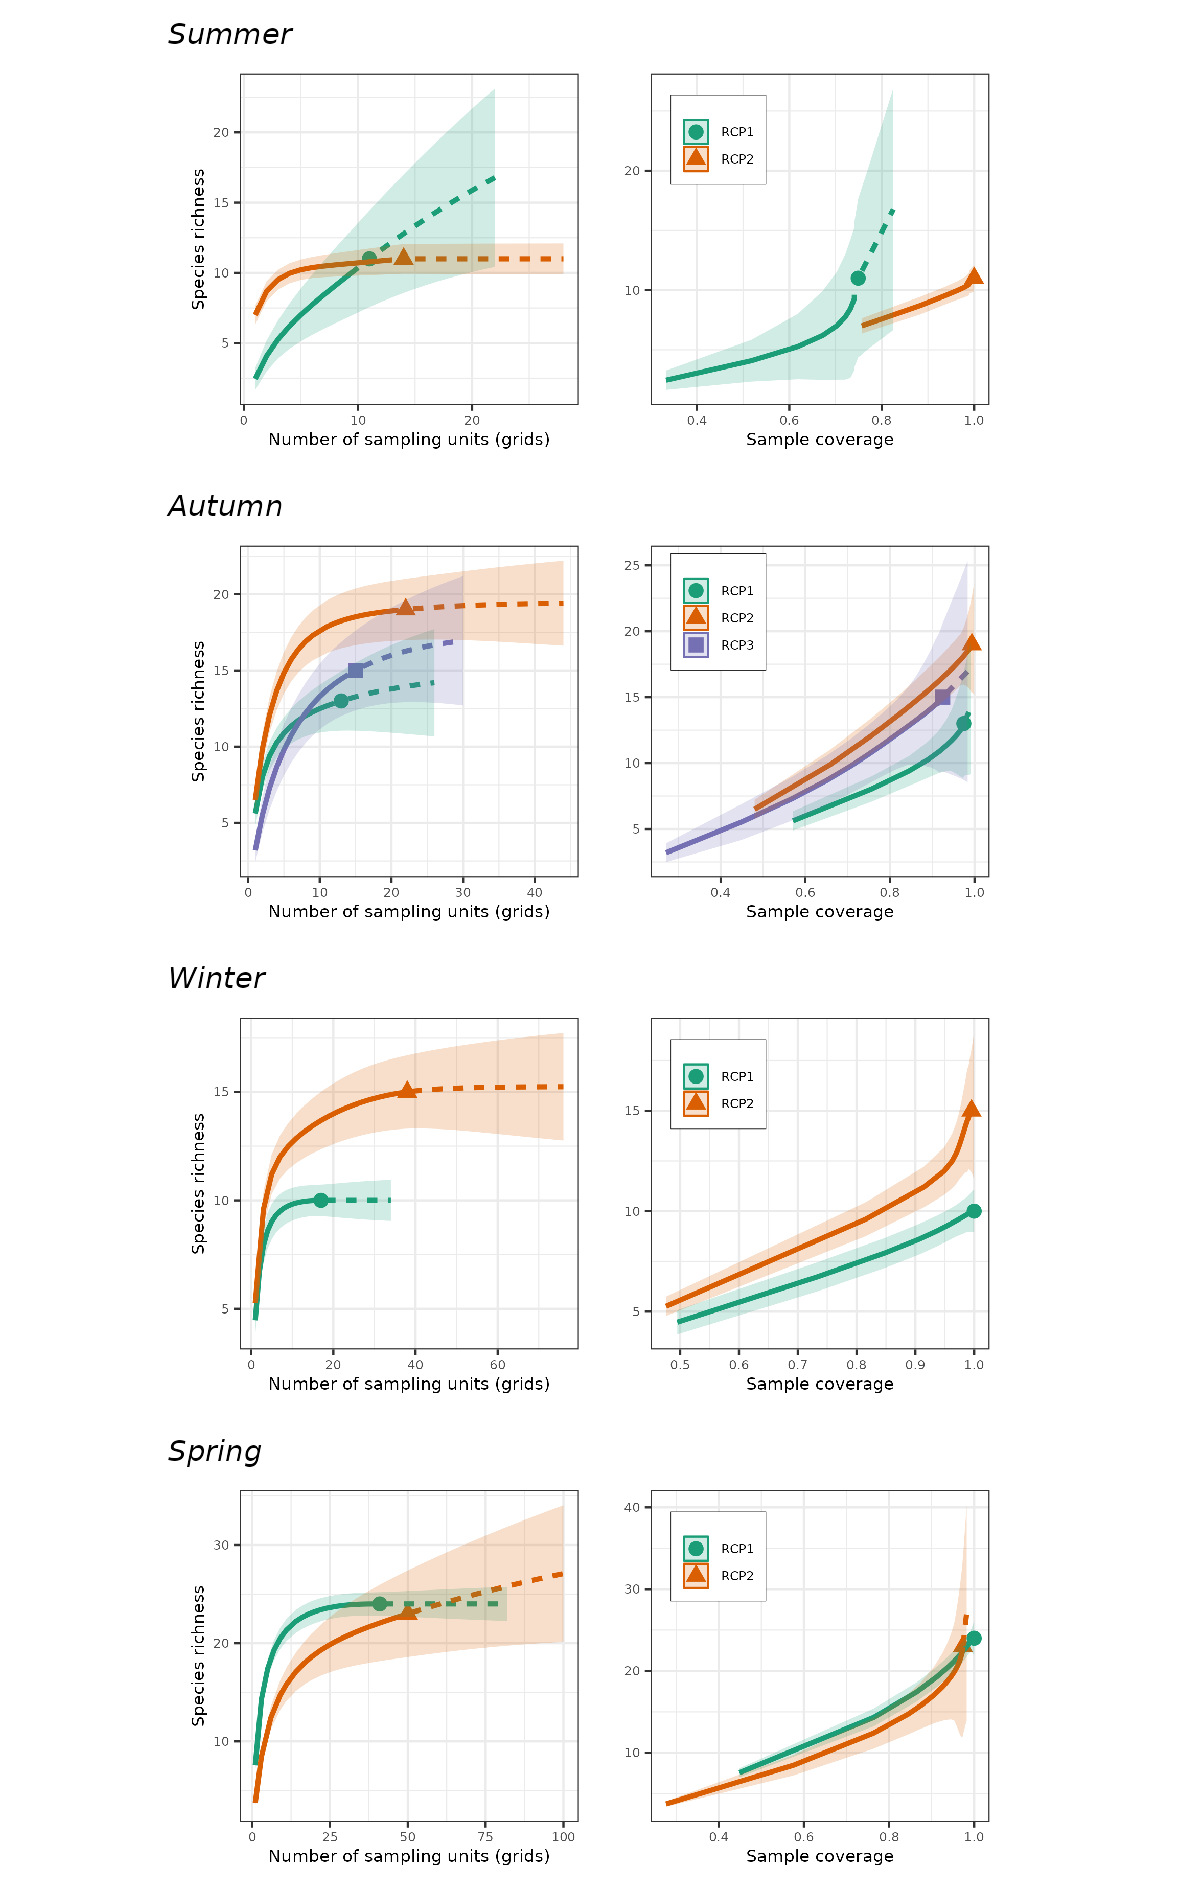
\includegraphics{../results/FigS8_iNEXT.png}
\caption{\textbf{Figure S8.} Diversity curve (alpha diversity) and
sample coverage for each assemblage (Region of Common Profile; RCP) from
each presence-absence seasonal model.}
\end{figure}

\newpage

\hypertarget{references}{%
\section*{References}\label{references}}
\addcontentsline{toc}{section}{References}

\hypertarget{refs}{}
\begin{CSLReferences}{1}{0}
\leavevmode\vadjust pre{\hypertarget{ref-mapview}{}}%
Appelhans, T., Detsch, F., Reudenbach, C., \& Woellauer, S. (2022).
\emph{Mapview: Interactive viewing of spatial data in r}.
\url{https://CRAN.R-project.org/package=mapview}

\leavevmode\vadjust pre{\hypertarget{ref-sp2}{}}%
Bivand, R. S., Pebesma, E., \& Gomez-Rubio, V. (2013). \emph{Applied
spatial data analysis with {R}, second edition}. Springer, NY.
\url{https://asdar-book.org/}

\leavevmode\vadjust pre{\hypertarget{ref-hadsstr}{}}%
Byrnes, J., \& Dunic, J. (2017). \emph{hadsstR: R library for working
with HadSST data}. \url{https://github.com/jebyrnes/hadsstR}

\leavevmode\vadjust pre{\hypertarget{ref-rerddap}{}}%
Chamberlain, S. (2023). \emph{Rerddap: General purpose client for
'ERDDAP' servers}. \url{https://CRAN.R-project.org/package=rerddap}

\leavevmode\vadjust pre{\hypertarget{ref-ggspatial}{}}%
Dunnington, D. (2022). \emph{Ggspatial: Spatial data framework for
ggplot2}. \url{https://CRAN.R-project.org/package=ggspatial}

\leavevmode\vadjust pre{\hypertarget{ref-lubridate}{}}%
Grolemund, G., \& Wickham, H. (2011). Dates and times made easy with
{lubridate}. \emph{Journal of Statistical Software}, \emph{40}(3),
1--25. \url{https://www.jstatsoft.org/v40/i03/}

\leavevmode\vadjust pre{\hypertarget{ref-raster}{}}%
Hijmans, R. J. (2022a). \emph{Raster: Geographic data analysis and
modeling}. \url{https://CRAN.R-project.org/package=raster}

\leavevmode\vadjust pre{\hypertarget{ref-terra}{}}%
Hijmans, R. J. (2022b). \emph{Terra: Spatial data analysis}.
\url{https://CRAN.R-project.org/package=terra}

\leavevmode\vadjust pre{\hypertarget{ref-rnaturalearth}{}}%
Massicotte, P., \& South, A. (2023). \emph{Rnaturalearth: World map data
from natural earth}.
\url{https://CRAN.R-project.org/package=rnaturalearth}

\leavevmode\vadjust pre{\hypertarget{ref-rerddapXtracto}{}}%
Mendelssohn, R. (2022). \emph{rerddapXtracto: Extracts environmental
data from 'ERDDAP' web services}.
\url{https://CRAN.R-project.org/package=rerddapXtracto}

\leavevmode\vadjust pre{\hypertarget{ref-tibble}{}}%
Müller, K., \& Wickham, H. (2023). \emph{Tibble: Simple data frames}.
\url{https://CRAN.R-project.org/package=tibble}

\leavevmode\vadjust pre{\hypertarget{ref-rcolorbrewer}{}}%
Neuwirth, E. (2022). \emph{RColorBrewer: ColorBrewer palettes}.
\url{https://CRAN.R-project.org/package=RColorBrewer}

\leavevmode\vadjust pre{\hypertarget{ref-sf}{}}%
Pebesma, E. (2018). {Simple features for R: standardized support for
spatial vector data}. \emph{{The R Journal}}, \emph{10}(1), 439--446.
\url{https://doi.org/10.32614/RJ-2018-009}

\leavevmode\vadjust pre{\hypertarget{ref-sp1}{}}%
Pebesma, E. J., \& Bivand, R. S. (2005). Classes and methods for spatial
data in {R}. \emph{R News}, \emph{5}(2), 9--13.
\url{https://CRAN.R-project.org/doc/Rnews/}

\leavevmode\vadjust pre{\hypertarget{ref-patchwork}{}}%
Pedersen, T. L. (2022). \emph{Patchwork: The composer of plots}.
\url{https://CRAN.R-project.org/package=patchwork}

\leavevmode\vadjust pre{\hypertarget{ref-corrplot2021}{}}%
Wei, T., \& Simko, V. (2021). \emph{R package 'corrplot': Visualization
of a correlation matrix}. \url{https://github.com/taiyun/corrplot}

\leavevmode\vadjust pre{\hypertarget{ref-plyr}{}}%
Wickham, H. (2011). The split-apply-combine strategy for data analysis.
\emph{Journal of Statistical Software}, \emph{40}(1), 1--29.
\url{https://www.jstatsoft.org/v40/i01/}

\leavevmode\vadjust pre{\hypertarget{ref-ggplot2}{}}%
Wickham, H. (2016). \emph{ggplot2: Elegant graphics for data analysis}.
Springer-Verlag New York. \url{https://ggplot2.tidyverse.org}

\leavevmode\vadjust pre{\hypertarget{ref-stringr}{}}%
Wickham, H. (2022). \emph{Stringr: Simple, consistent wrappers for
common string operations}.
\url{https://CRAN.R-project.org/package=stringr}

\leavevmode\vadjust pre{\hypertarget{ref-dplyr}{}}%
Wickham, H., François, R., Henry, L., Müller, K., \& Vaughan, D. (2023).
\emph{Dplyr: A grammar of data manipulation}.
\url{https://CRAN.R-project.org/package=dplyr}

\leavevmode\vadjust pre{\hypertarget{ref-purrr}{}}%
Wickham, H., \& Henry, L. (2023). \emph{Purrr: Functional programming
tools}. \url{https://CRAN.R-project.org/package=purrr}

\leavevmode\vadjust pre{\hypertarget{ref-readr}{}}%
Wickham, H., Hester, J., \& Bryan, J. (2023). \emph{Readr: Read
rectangular text data}. \url{https://CRAN.R-project.org/package=readr}

\leavevmode\vadjust pre{\hypertarget{ref-tidyr}{}}%
Wickham, H., Vaughan, D., \& Girlich, M. (2023). \emph{Tidyr: Tidy messy
data}. \url{https://CRAN.R-project.org/package=tidyr}

\end{CSLReferences}

\end{document}
